%% bare_conf.tex
%% V1.3
%% 2007/01/11
%% by Michael Shell
%% See:
%% http://www.michaelshell.org/
%% for current contact information.
%%
%% This is a skeleton file demonstrating the use of IEEEtran.cls
%% (requires IEEEtran.cls version 1.7 or later) with an IEEE conference paper.
%%
%% Support sites:
%% http://www.michaelshell.org/tex/ieeetran/
%% http://www.ctan.org/tex-archive/macros/latex/contrib/IEEEtran/
%% and
%% http://www.ieee.org/

%%*************************************************************************
%% Legal Notice:
%% This code is offered as-is without any warranty either expressed or
%% implied; without even the implied warranty of MERCHANTABILITY or
%% FITNESS FOR A PARTICULAR PURPOSE! 
%% User assumes all risk.
%% In no event shall IEEE or any contributor to this code be liable for
%% any damages or losses, including, but not limited to, incidental,
%% consequential, or any other damages, resulting from the use or misuse
%% of any information contained here.
%%
%% All comments are the opinions of their respective authors and are not
%% necessarily endorsed by the IEEE.
%%
%% This work is distributed under the LaTeX Project Public License (LPPL)
%% ( http://www.latex-project.org/ ) version 1.3, and may be freely used,
%% distributed and modified. A copy of the LPPL, version 1.3, is included
%% in the base LaTeX documentation of all distributions of LaTeX released
%% 2003/12/01 or later.
%% Retain all contribution notices and credits.
%% ** Modified files should be clearly indicated as such, including  **
%% ** renaming them and changing author support contact information. **
%%
%% File list of work: IEEEtran.cls, IEEEtran_HOWTO.pdf, bare_adv.tex,
%%                    bare_conf.tex, bare_jrnl.tex, bare_jrnl_compsoc.tex
%%*************************************************************************

% *** Authors should verify (and, if needed, correct) their LaTeX system  ***
% *** with the testflow diagnostic prior to trusting their LaTeX platform ***
% *** with production work. IEEE's font choices can trigger bugs that do  ***
% *** not appear when using other class files.                            ***
% The testflow support page is at:
% http://www.michaelshell.org/tex/testflow/



% Note that the a4paper option is mainly intended so that authors in
% countries using A4 can easily print to A4 and see how their papers will
% look in print - the typesetting of the document will not typically be
% affected with changes in paper size (but the bottom and side margins will).
% Use the testflow package mentioned above to verify correct handling of
% both paper sizes by the user's LaTeX system.
%
% Also note that the "draftcls" or "draftclsnofoot", not "draft", option
% should be used if it is desired that the figures are to be displayed in
% draft mode.
%
\documentclass[10pt,conference,compsocconf]{IEEEtran}
%\documentclass[10pt]{IEEEtran}
\usepackage{times}

\usepackage{caption}
\captionsetup{font=footnotesize,justification=centering,labelsep=period}

% Add the compsoc option for Computer Society conferences.
%
% If IEEEtran.cls has not been installed into the LaTeX system files,
% manually specify the path to it like:
% \documentclass[conference]{../sty/IEEEtran}





% Some very useful LaTeX packages include:
% (uncomment the ones you want to load)


% *** MISC UTILITY PACKAGES ***
%
%\usepackage{ifpdf}
% Heiko Oberdiek's ifpdf.sty is very useful if you need conditional
% compilation based on whether the output is pdf or dvi.
% usage:
% \ifpdf
%   % pdf code
% \else
%   % dvi code
% \fi
% The latest version of ifpdf.sty can be obtained from:
% http://www.ctan.org/tex-archive/macros/latex/contrib/oberdiek/
% Also, note that IEEEtran.cls V1.7 and later provides a builtin
% \ifCLASSINFOpdf conditional that works the same way.
% When switching from latex to pdflatex and vice-versa, the compiler may
% have to be run twice to clear warning/error messages.






% *** CITATION PACKAGES ***
%
%\usepackage{cite}
% cite.sty was written by Donald Arseneau
% V1.6 and later of IEEEtran pre-defines the format of the cite.sty package
% \cite{} output to follow that of IEEE. Loading the cite package will
% result in citation numbers being automatically sorted and properly
% "compressed/ranged". e.g., [1], [9], [2], [7], [5], [6] without using
% cite.sty will become [1], [2], [5]--[7], [9] using cite.sty. cite.sty's
% \cite will automatically add leading space, if needed. Use cite.sty's
% noadjust option (cite.sty V3.8 and later) if you want to turn this off.
% cite.sty is already installed on most LaTeX systems. Be sure and use
% version 4.0 (2003-05-27) and later if using hyperref.sty. cite.sty does
% not currently provide for hyperlinked citations.
% The latest version can be obtained at:
% http://www.ctan.org/tex-archive/macros/latex/contrib/cite/
% The documentation is contained in the cite.sty file itself.






% *** GRAPHICS RELATED PACKAGES ***
%
\ifCLASSINFOpdf
  % \usepackage[pdftex]{graphicx}
  % declare the path(s) where your graphic files are
  % \graphicspath{{../pdf/}{../jpeg/}}
  % and their extensions so you won't have to specify these with
  % every instance of \includegraphics
  % \DeclareGraphicsExtensions{.pdf,.jpeg,.png}
\else
  % or other class option (dvipsone, dvipdf, if not using dvips). graphicx
  % will default to the driver specified in the system graphics.cfg if no
  % driver is specified.
  % \usepackage[dvips]{graphicx}
  % declare the path(s) where your graphic files are
  % \graphicspath{{../eps/}}
  % and their extensions so you won't have to specify these with
  % every instance of \includegraphics
  % \DeclareGraphicsExtensions{.eps}
\fi
% graphicx was written by David Carlisle and Sebastian Rahtz. It is
% required if you want graphics, photos, etc. graphicx.sty is already
% installed on most LaTeX systems. The latest version and documentation can
% be obtained at: 
% http://www.ctan.org/tex-archive/macros/latex/required/graphics/
% Another good source of documentation is "Using Imported Graphics in
% LaTeX2e" by Keith Reckdahl which can be found as epslatex.ps or
% epslatex.pdf at: http://www.ctan.org/tex-archive/info/
%
% latex, and pdflatex in dvi mode, support graphics in encapsulated
% postscript (.eps) format. pdflatex in pdf mode supports graphics
% in .pdf, .jpeg, .png and .mps (metapost) formats. Users should ensure
% that all non-photo figures use a vector format (.eps, .pdf, .mps) and
% not a bitmapped formats (.jpeg, .png). IEEE frowns on bitmapped formats
% which can result in "jaggedy"/blurry rendering of lines and letters as
% well as large increases in file sizes.
%
% You can find documentation about the pdfTeX application at:
% http://www.tug.org/applications/pdftex





% *** MATH PACKAGES ***
%
\usepackage[cmex10]{amsmath}
% A popular package from the American Mathematical Society that provides
% many useful and powerful commands for dealing with mathematics. If using
% it, be sure to load this package with the cmex10 option to ensure that
% only type 1 fonts will utilized at all point sizes. Without this option,
% it is possible that some math symbols, particularly those within
% footnotes, will be rendered in bitmap form which will result in a
% document that can not be IEEE Xplore compliant!
%
% Also, note that the amsmath package sets \interdisplaylinepenalty to 10000
% thus preventing page breaks from occurring within multiline equations. Use:
%\interdisplaylinepenalty=2500
% after loading amsmath to restore such page breaks as IEEEtran.cls normally
% does. amsmath.sty is already installed on most LaTeX systems. The latest
% version and documentation can be obtained at:
% http://www.ctan.org/tex-archive/macros/latex/required/amslatex/math/





% *** SPECIALIZED LIST PACKAGES ***
%
%\usepackage{algorithmic}
% algorithmic.sty was written by Peter Williams and Rogerio Brito.
% This package provides an algorithmic environment fo describing algorithms.
% You can use the algorithmic environment in-text or within a figure
% environment to provide for a floating algorithm. Do NOT use the algorithm
% floating environment provided by algorithm.sty (by the same authors) or
% algorithm2e.sty (by Christophe Fiorio) as IEEE does not use dedicated
% algorithm float types and packages that provide these will not provide
% correct IEEE style captions. The latest version and documentation of
% algorithmic.sty can be obtained at:
% http://www.ctan.org/tex-archive/macros/latex/contrib/algorithms/
% There is also a support site at:
% http://algorithms.berlios.de/index.html
% Also of interest may be the (relatively newer and more customizable)
% algorithmicx.sty package by Szasz Janos:
% http://www.ctan.org/tex-archive/macros/latex/contrib/algorithmicx/




% *** ALIGNMENT PACKAGES ***
%
%\usepackage{array}
% Frank Mittelbach's and David Carlisle's array.sty patches and improves
% the standard LaTeX2e array and tabular environments to provide better
% appearance and additional user controls. As the default LaTeX2e table
% generation code is lacking to the point of almost being broken with
% respect to the quality of the end results, all users are strongly
% advised to use an enhanced (at the very least that provided by array.sty)
% set of table tools. array.sty is already installed on most systems. The
% latest version and documentation can be obtained at:
% http://www.ctan.org/tex-archive/macros/latex/required/tools/


%\usepackage{mdwmath}
%\usepackage{mdwtab}
% Also highly recommended is Mark Wooding's extremely powerful MDW tools,
% especially mdwmath.sty and mdwtab.sty which are used to format equations
% and tables, respectively. The MDWtools set is already installed on most
% LaTeX systems. The lastest version and documentation is available at:
% http://www.ctan.org/tex-archive/macros/latex/contrib/mdwtools/


% IEEEtran contains the IEEEeqnarray family of commands that can be used to
% generate multiline equations as well as matrices, tables, etc., of high
% quality.


%\usepackage{eqparbox}
% Also of notable interest is Scott Pakin's eqparbox package for creating
% (automatically sized) equal width boxes - aka "natural width parboxes".
% Available at:
% http://www.ctan.org/tex-archive/macros/latex/contrib/eqparbox/





% *** SUBFIGURE PACKAGES ***
%\usepackage[tight,footnotesize]{subfigure}
% subfigure.sty was written by Steven Douglas Cochran. This package makes it
% easy to put subfigures in your figures. e.g., "Figure 1a and 1b". For IEEE
% work, it is a good idea to load it with the tight package option to reduce
% the amount of white space around the subfigures. subfigure.sty is already
% installed on most LaTeX systems. The latest version and documentation can
% be obtained at:
% http://www.ctan.org/tex-archive/obsolete/macros/latex/contrib/subfigure/
% subfigure.sty has been superceeded by subfig.sty.



%\usepackage[caption=false]{caption}
%\usepackage[font=footnotesize]{subfig}
% subfig.sty, also written by Steven Douglas Cochran, is the modern
% replacement for subfigure.sty. However, subfig.sty requires and
% automatically loads Axel Sommerfeldt's caption.sty which will override
% IEEEtran.cls handling of captions and this will result in nonIEEE style
% figure/table captions. To prevent this problem, be sure and preload
% caption.sty with its "caption=false" package option. This is will preserve
% IEEEtran.cls handing of captions. Version 1.3 (2005/06/28) and later 
% (recommended due to many improvements over 1.2) of subfig.sty supports
% the caption=false option directly:
%\usepackage[caption=false,font=footnotesize]{subfig}
%
% The latest version and documentation can be obtained at:
% http://www.ctan.org/tex-archive/macros/latex/contrib/subfig/
% The latest version and documentation of caption.sty can be obtained at:
% http://www.ctan.org/tex-archive/macros/latex/contrib/caption/




% *** FLOAT PACKAGES ***
%
%\usepackage{fixltx2e}
% fixltx2e, the successor to the earlier fix2col.sty, was written by
% Frank Mittelbach and David Carlisle. This package corrects a few problems
% in the LaTeX2e kernel, the most notable of which is that in current
% LaTeX2e releases, the ordering of single and double column floats is not
% guaranteed to be preserved. Thus, an unpatched LaTeX2e can allow a
% single column figure to be placed prior to an earlier double column
% figure. The latest version and documentation can be found at:
% http://www.ctan.org/tex-archive/macros/latex/base/



%\usepackage{stfloats}
% stfloats.sty was written by Sigitas Tolusis. This package gives LaTeX2e
% the ability to do double column floats at the bottom of the page as well
% as the top. (e.g., "\begin{figure*}[!b]" is not normally possible in
% LaTeX2e). It also provides a command:
%\fnbelowfloat
% to enable the placement of footnotes below bottom floats (the standard
% LaTeX2e kernel puts them above bottom floats). This is an invasive package
% which rewrites many portions of the LaTeX2e float routines. It may not work
% with other packages that modify the LaTeX2e float routines. The latest
% version and documentation can be obtained at:
% http://www.ctan.org/tex-archive/macros/latex/contrib/sttools/
% Documentation is contained in the stfloats.sty comments as well as in the
% presfull.pdf file. Do not use the stfloats baselinefloat ability as IEEE
% does not allow \baselineskip to stretch. Authors submitting work to the
% IEEE should note that IEEE rarely uses double column equations and
% that authors should try to avoid such use. Do not be tempted to use the
% cuted.sty or midfloat.sty packages (also by Sigitas Tolusis) as IEEE does
% not format its papers in such ways.





% *** PDF, URL AND HYPERLINK PACKAGES ***
%
%\usepackage{url}
% url.sty was written by Donald Arseneau. It provides better support for
% handling and breaking URLs. url.sty is already installed on most LaTeX
% systems. The latest version can be obtained at:
% http://www.ctan.org/tex-archive/macros/latex/contrib/misc/
% Read the url.sty source comments for usage information. Basically,
% \url{my_url_here}.





% *** Do not adjust lengths that control margins, column widths, etc. ***
% *** Do not use packages that alter fonts (such as pslatex).         ***
% There should be no need to do such things with IEEEtran.cls V1.6 and later.
% (Unless specifically asked to do so by the journal or conference you plan
% to submit to, of course. )





% ---------- my stuff ----------
\usepackage{tikz}
\usetikzlibrary{arrows}
\usetikzlibrary{shapes}
\usetikzlibrary{positioning}
\usetikzlibrary{backgrounds}
\usetikzlibrary{calc}
\usepackage{3dplot}
\usetikzlibrary{trees}
\usetikzlibrary{chains,fit,shapes,intersections}

\usepackage[plain]{algorithm}
%\usepackage[noend]{algorithmic}
\usepackage{algorithmic}

%\usepackage[]{algorithm2e}
%%\usepackage[hang]{subfigure}
\usepackage[nooneline]{subfigure}
\usepackage{subfigure}

%\usepackage{amsmath}

\newcommand{\ga}{{\gamma}}



%\newcommand{\xv}{\mbox{\boldmath $x$}} % funker ikke lenger...!?

\newcommand{\bv}{\mathbf{b}}
\newcommand{\cv}{\mathbf{c}}
\newcommand{\dv}{\mathbf{d}}
\newcommand{\ev}{\mathbf{e}}
\newcommand{\mv}{\mathbf{m}}
\newcommand{\pv}{\mathbf{p}}
\newcommand{\sv}{\mathbf{s}}
\newcommand{\uv}{\mathbf{u}}
\newcommand{\vv}{\mathbf{v}}
\newcommand{\xv}{\mathbf{x}}		% Works, but seems more Roman than italics!

\newcommand{\ub}{\bar{u}}

\newcommand{\evh}{\hat{\mathbf{e}}}

\newcommand{\Ev}{\mathbf{E}}
\newcommand{\Fv}{\mathbf{F}}
\newcommand{\Tv}{\mathbf{T}}
\newcommand{\Nv}{\mathbf{N}}
\newcommand{\Bv}{\mathbf{B}}

\newcommand{\Tvh}{\hat{\mathbf{T}}}
\newcommand{\Nvh}{\hat{\mathbf{N}}}
\newcommand{\Bvh}{\hat{\mathbf{B}}}

\newcommand{\Tvb}{\bar{\mathbf{T}}}
\newcommand{\Nvb}{\bar{\mathbf{N}}}
\newcommand{\Bvb}{\bar{\mathbf{B}}}

%\newcommand{\Tvd}{\dot{\mathbf{T}}}
\newcommand{\Tvd}{\mathbf{T}'}

\newcommand{\zev}{\mathbf{0}}

\newcommand{\ra}{\rightarrow}
\newcommand{\la}{\leftarrow}

%\newcommand{\gav}{\mathbf{\gamma}} % funker heller ikke!
\newcommand{\gav}{\boldsymbol{\gamma}} % Works only when bm.sty is used. If it is not, we get an ordinary symbol, but no warning/error!
\newcommand{\nuv}{\boldsymbol{\nu}}
\newcommand{\nuvh}{\boldsymbol{\nu}}

\newcommand{\xvv}{\boldsymbol{x}}	% Strange. This looks like a ``poor mans bold'', i.e., a couple of superimposed
	                                % and slightly offset x'es...

\newcommand{\ie}{{\em i.e.}}
\newcommand{\eg}{{\em e.g.}}
\newcommand{\etal}{{\em et~al.}}


% ------------------------------
















% correct bad hyphenation here
\hyphenation{op-tical net-works semi-conduc-tor}

%\parskip 6pt plus 2pt minus 1pt
\parskip 3pt plus 2pt minus 1pt

\pagestyle{empty}
\begin{document}
\pagenumbering{gobble}
%
% paper title
% can use linebreaks \\ within to get better formatting as desired
\title{\textbf{\Large Hybrid Client/Server Rendering with Automatic Proxy Model Generation}\\[0.2ex]}

% author names and affiliations
% use a multiple column layout for up to three different
% affiliations

%\author[J.\,O. Nygaard \& J. Mikkelsen]
%       {J.\,O. Nygaard$^{1}$
%        and J. Mikkelsen$^{1}$
%        \\
%         $^1$SINTEF ICT, Applied Mathematics, Norway
%       }





\author{\IEEEauthorblockN{~\\[-0.4ex]\large Jens Olav Nygaard\\[0.3ex]\normalsize}
\IEEEauthorblockA{SINTEF Digital\\
Applied Mathematics\\
Norway\\
Email: {\tt Jens.O.Nygaard@sintef.no}}
\and
\IEEEauthorblockN{~\\[-0.4ex]\large Jon Mikkelsen Hjelmervik\\[0.3ex]\normalsize}
\IEEEauthorblockA{SINTEF Digital\\
Applied Mathematics\\
Norway\\
Email: {\tt Jon.M.Hjelmervik@sintef.no}}}

% conference papers do not typically use \thanks and this command
% is locked out in conference mode. If really needed, such as for
% the acknowledgment of grants, issue a \IEEEoverridecommandlockouts
% after \documentclass

% for over three affiliations, or if they all won't fit within the width
% of the page, use this alternative format:
% 
%\author{\IEEEauthorblockN{Michael Shell\IEEEauthorrefmark{1},
%Homer Simpson\IEEEauthorrefmark{2},
%James Kirk\IEEEauthorrefmark{3}, 
%Montgomery Scott\IEEEauthorrefmark{3} and
%Eldon Tyrell\IEEEauthorrefmark{4}}
%\IEEEauthorblockA{\IEEEauthorrefmark{1}School of Electrical and Computer Engineering\\
%Georgia Institute of Technology,
%Atlanta, Georgia 30332--0250\\ Email: see http://www.michaelshell.org/contact.html}
%\IEEEauthorblockA{\IEEEauthorrefmark{2}Twentieth Century Fox, Springfield, USA\\
%Email: homer@thesimpsons.com}
%\IEEEauthorblockA{\IEEEauthorrefmark{3}Starfleet Academy, San Francisco, California 96678-2391\\
%Telephone: (800) 555--1212, Fax: (888) 555--1212}
%\IEEEauthorblockA{\IEEEauthorrefmark{4}Tyrell Inc., 123 Replicant Street, Los Angeles, California 90210--4321}}




% use for special paper notices
%\IEEEspecialpapernotice{(Invited Paper)}




% make the title area
%\maketitle

%\teaser
%{
%  \centering
%  \subfigure[Server-rendered (OpenGL)]{
%    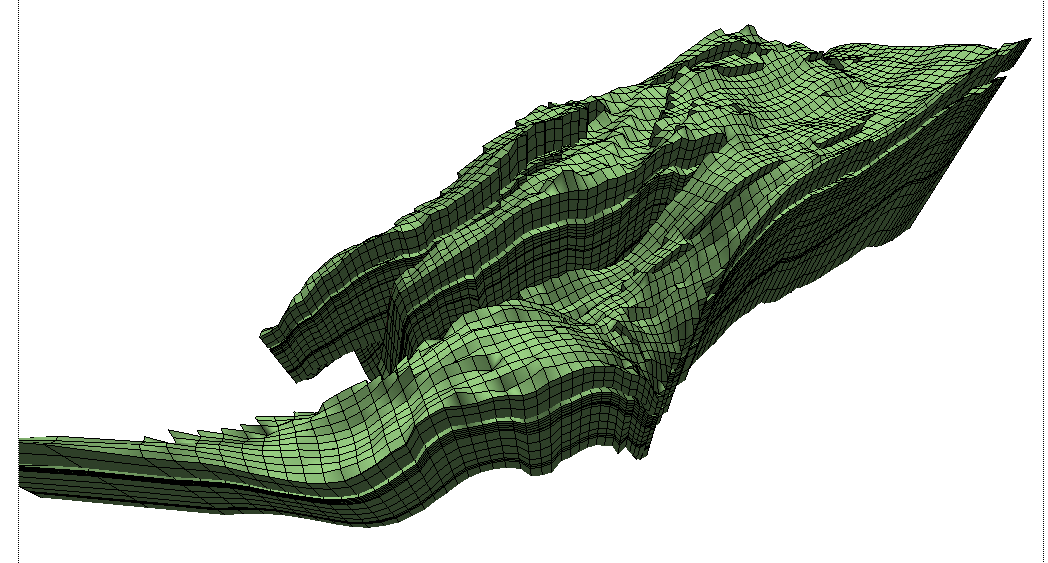
\includegraphics[width=0.32\linewidth, trim={1cm 1cm 1cm 1cm}, clip]{frviewb1.png}
%  }
%  \subfigure[Client-rendered (WebGL)]{
%    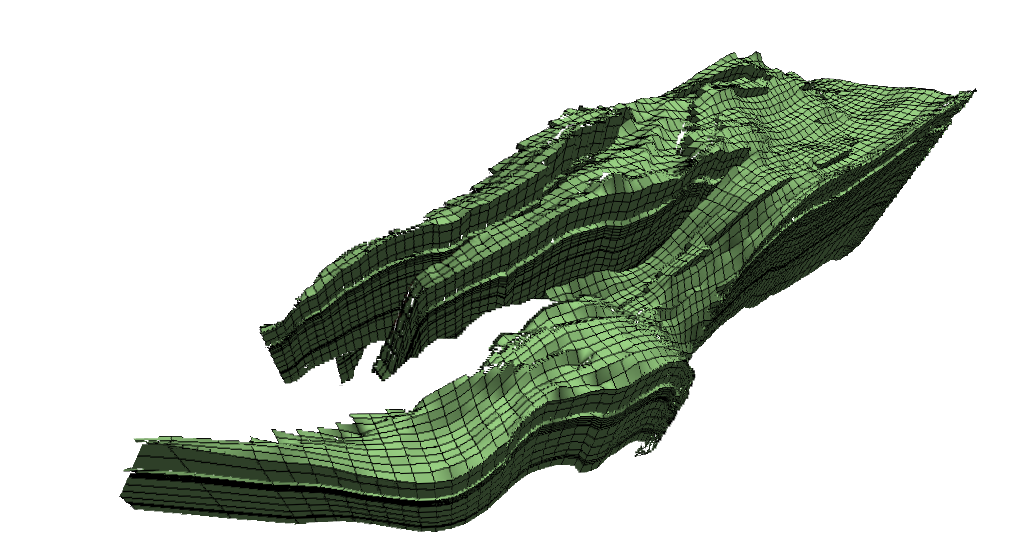
\includegraphics[width=0.32\linewidth, trim={0 1cm 0 1.5cm}, clip]{frviewb2.png}
%  }
%  \subfigure[Client-rendered (WebGL)]{
%    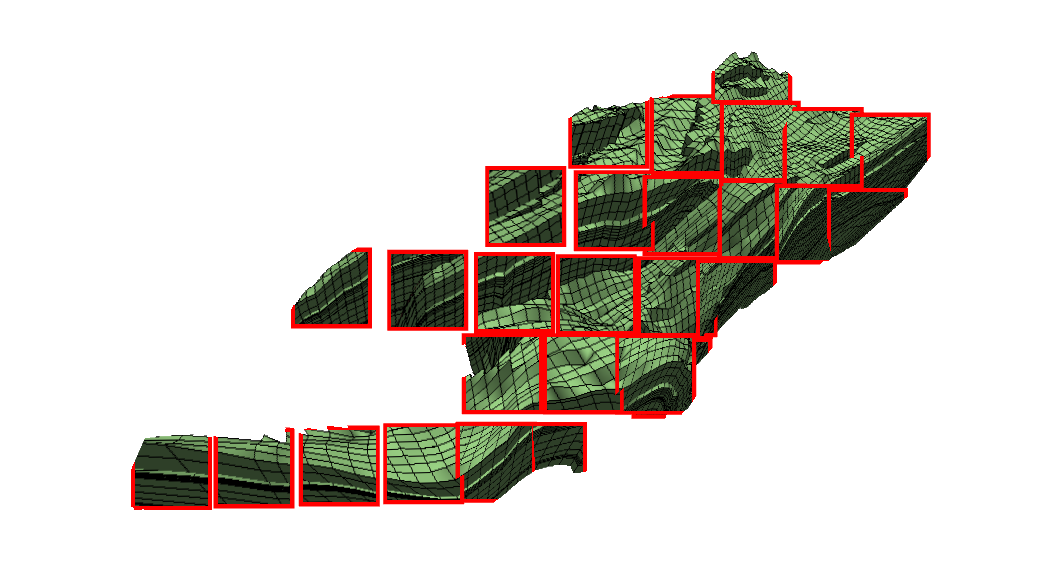
\includegraphics[width=0.32\linewidth, trim={0 1.5cm 0 2cm}, clip]{frviewb3.png}
%    % The trim params: left lower right upper
%  }
%  \caption{\label{fig:FRView} The oil reservoir viewer YYYY~\cite{cloudviz},
%  (name withheld for the double-blind review process) showing one
%  server-rendered and two client-rendered images of automatically generated and
%  slightly rotated proxy models.  For~(b), parameters are chosen to produce the
%  best possible image, and in~(c) we want to highlight artifacts and
%  implementational details. See the text for further discussion.}
%}



\twocolumn[{%
\renewcommand\twocolumn[1][]{#1}%
\maketitle
\begin{center}
    \centering
		\begin{tabular}[b]{ccc}
    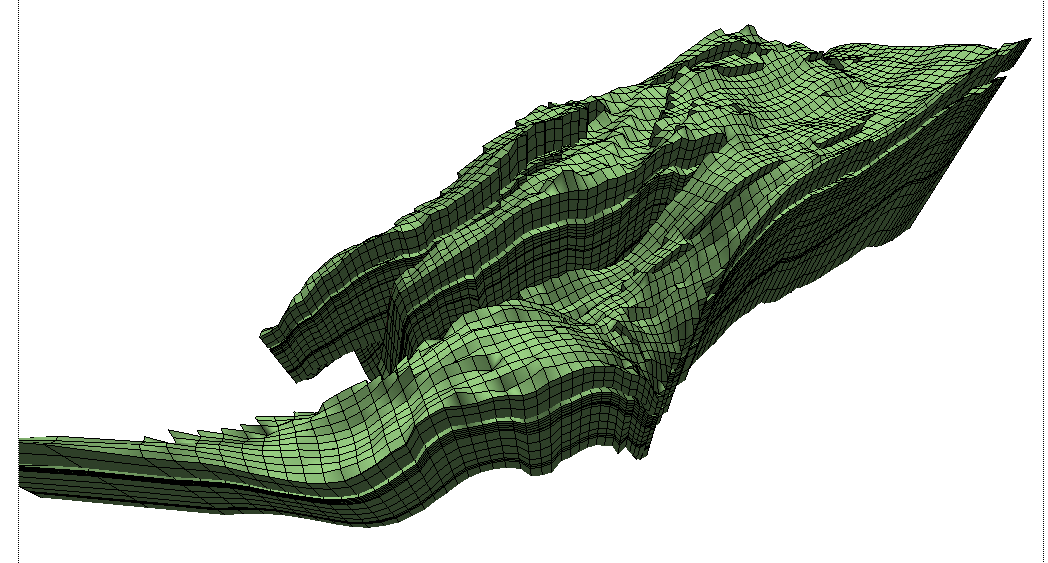
\includegraphics[width=0.32\linewidth, trim={1cm 1cm 1cm 1cm}, clip]{frviewb1.png} &
    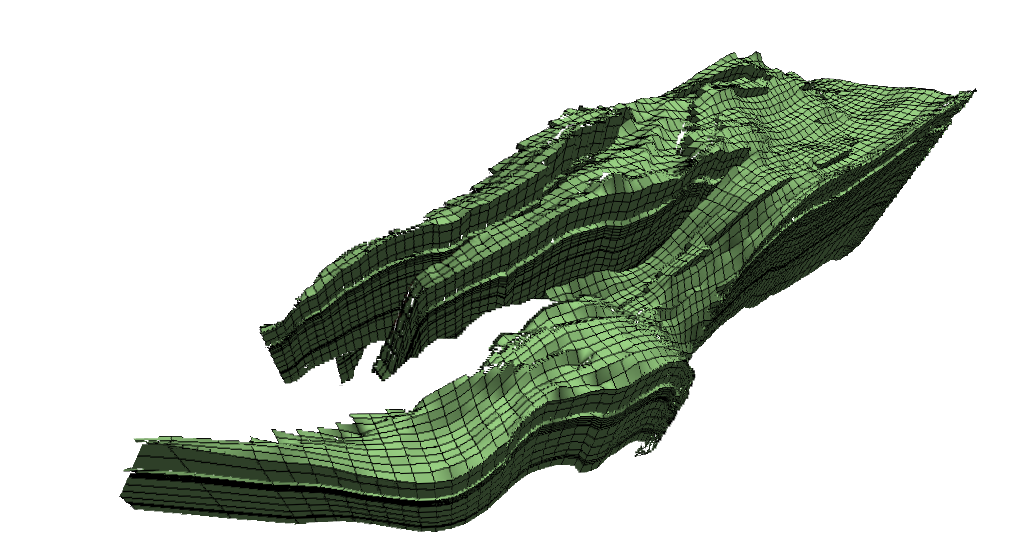
\includegraphics[width=0.32\linewidth, trim={0 1cm 0 1.5cm}, clip]{frviewb2.png} &
    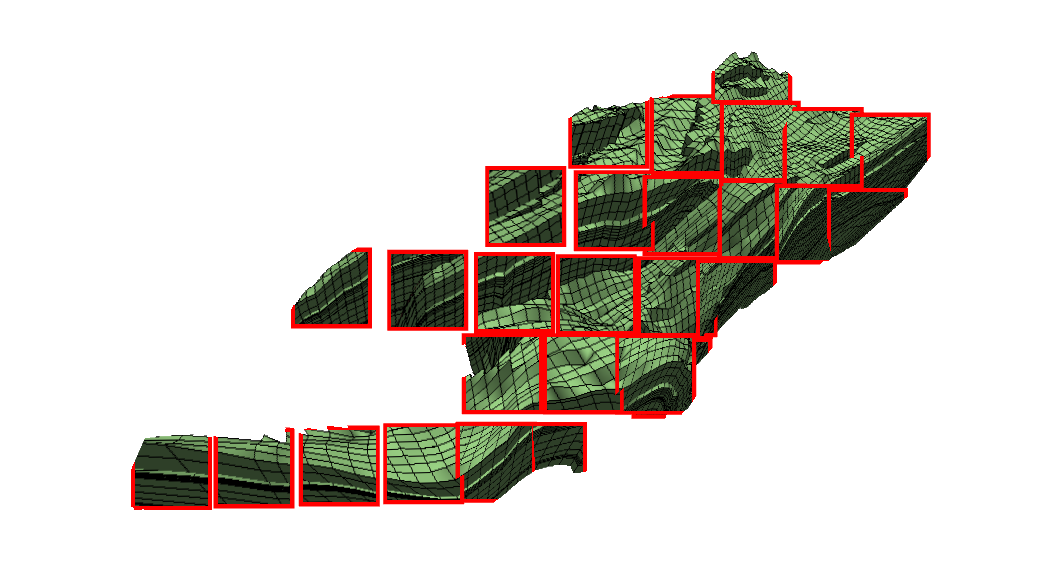
\includegraphics[width=0.32\linewidth, trim={0 1.5cm 0 2cm}, clip]{frviewb3.png} \\
		a) & b) & c)
		\end{tabular}
		\captionof{figure}{\label{fig:FRView} Oil reservoir viewer showing one
  server-rendered and two client-rendered images of automatically generated and
  slightly rotated proxy models.  For~(b), parameters are chosen to produce the
  best possible image, and in~(c) we want to highlight artifacts and
  implementational details. See the text for further discussion.}
%    \protect \label{fig:wfedesign} }
%    \captionof{figure}{Test caption}
\end{center}%
}]

%\begin{figure*}
%    % The star in \begin{figure*} makes the figure stretch across both columns.
%    \centering
%    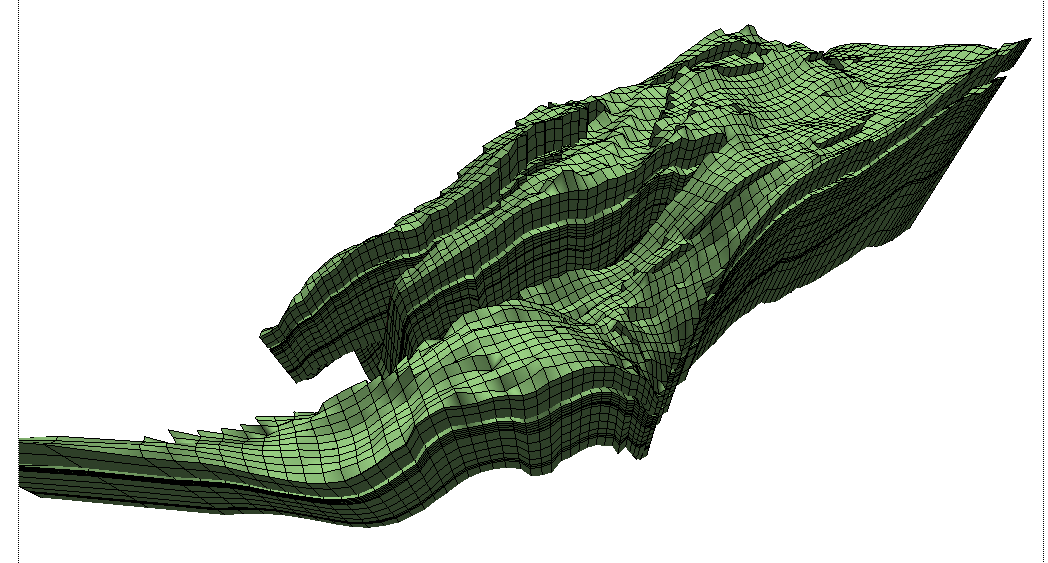
\includegraphics[width=0.99\linewidth]{frviewb1.png}
%    \caption{
%        %The graphical user interface of WFE, where dotted lines represent flow of services, while solid lines connect parameters from outputs to inputs.
%        The graphical user interface of Workflow Editor displays buttons to append services and to add code snippets for conditional branches, loops, parallel service execution (split), etc., as well as options for service %filtering. It also lets users add inputs and outputs to the workflow with appropriate buttons shown as I and O. The workflow is shown as a directed graph, where blue boxes represent single CloudFlow services, and dark green% boxes are sub-workflows. The execution order is represented by the dotted arrows, while data flow is visualized by solid lines, which connect output parameters from services to be input parameters of others.}
%    \protect \label{fig:wfedesign}
%\end{figure*}

%\teaser
%{
%  \centering
%  \subfigure[Server-rendered (OpenGL)]{
%    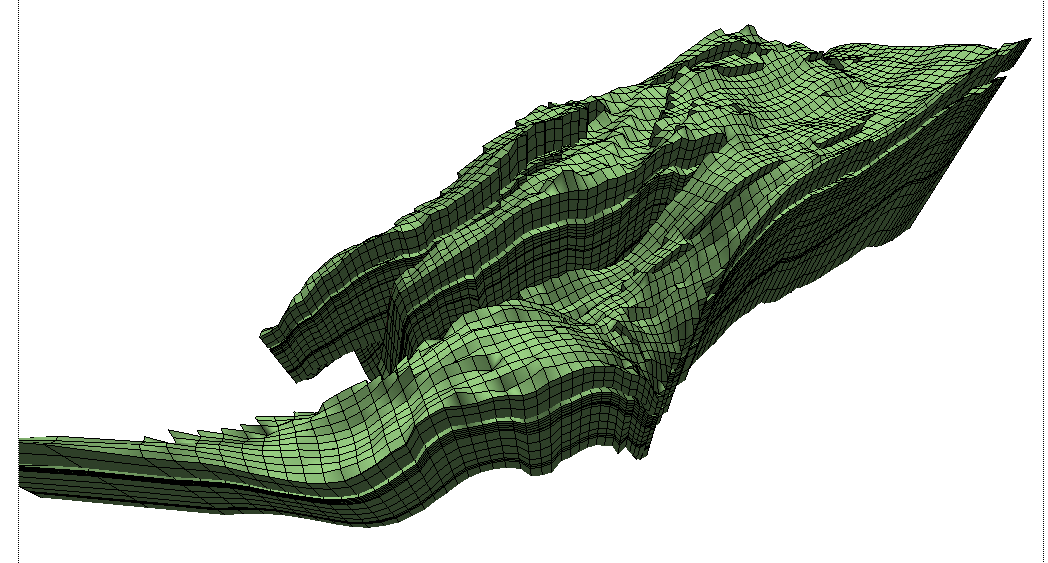
\includegraphics[width=0.32\linewidth, trim={1cm 1cm 1cm 1cm}, clip]{frviewb1.png}
%  }
%  \subfigure[Client-rendered (WebGL)]{
%    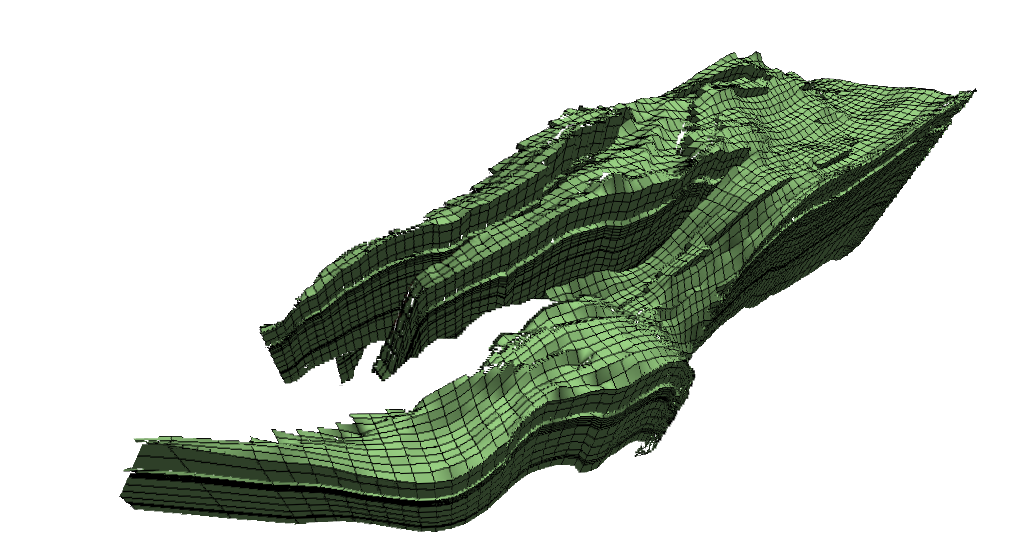
\includegraphics[width=0.32\linewidth, trim={0 1cm 0 1.5cm}, clip]{frviewb2.png}
%  }
%  \subfigure[Client-rendered (WebGL)]{
%    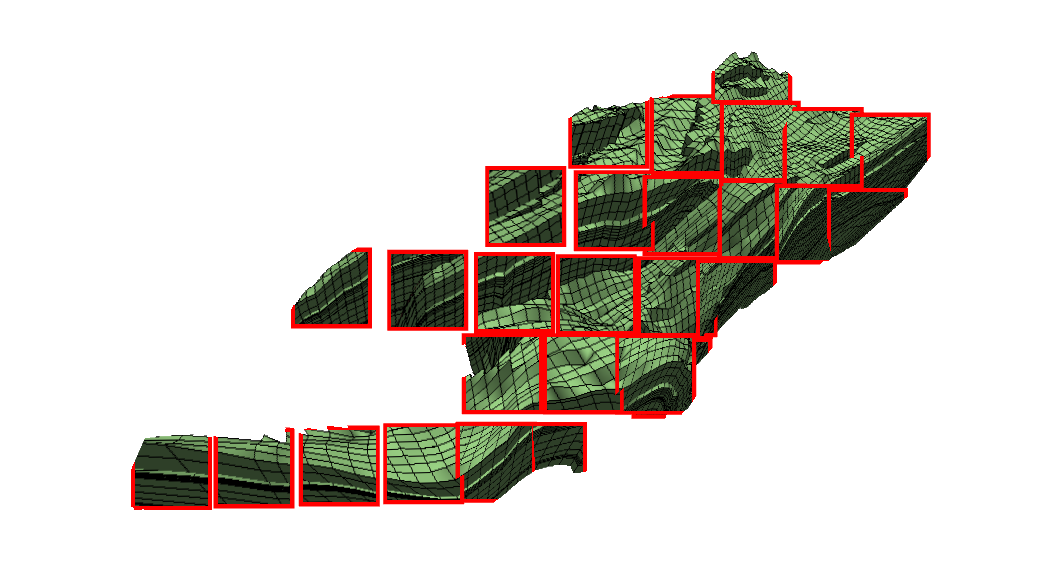
\includegraphics[width=0.32\linewidth, trim={0 1.5cm 0 2cm}, clip]{frviewb3.png}
%    % The trim params: left lower right upper
%  }
%  \caption{\label{fig:FRView} The oil reservoir viewer YYYY~\cite{cloudviz},
%  (name withheld for the double-blind review process) showing one
%  server-rendered and two client-rendered images of automatically generated and
%  slightly rotated proxy models.  For~(b), parameters are chosen to produce the
%  best possible image, and in~(c) we want to highlight artifacts and
%  implementational details. See the text for further discussion.}
%}


\begin{abstract}
%\boldmath
We describe an algorithm and implementation of automatic proxy model generation
for a client/server remote rendering setup. A {\em proxy model} is a
light-weight version of a main 3D model that is cheaper to render and
transfer. We automatically derive this from the main model. The client is
typically a tablet, for which we only assume availability of WebGL and
Javascript. The server makes use of OpenGL and a web server. When the rate of
received server-rendered images deteriorate, the client renders the proxy model,
which is computed from depth buffers bundled with rendered images from the
server. This algorithm requires little modification of the application itself.
\end{abstract}
% IEEEtran.cls defaults to using nonbold math in the Abstract.
% This preserves the distinction between vectors and scalars. However,
% if the conference you are submitting to favors bold math in the abstract,
% then you can use LaTeX's standard command \boldmath at the very start
% of the abstract to achieve this. Many IEEE journals/conferences frown on
% math in the abstract anyway.

% no keywords

\begin{IEEEkeywords}
Client-server; remote rendering; high latency; low bandwidth
\end{IEEEkeywords}



% For peer review papers, you can put extra information on the cover
% page as needed:
% \ifCLASSOPTIONpeerreview
% \begin{center} \bfseries EDICS Category: 3-BBND \end{center}
% \fi
%
% For peerreview papers, this IEEEtran command inserts a page break and
% creates the second title. It will be ignored for other modes.
\IEEEpeerreviewmaketitle



















%-------------------------------------------------------------------------
\section{Introduction}

Hand in hand with increasingly powerful rendering engines comes ever increasing
requirements on computational accuracy, power efficiency, data sizes, scaling
properties, etc. This is also reinforced by popular cloud-based approaches and
wireless usage patterns. An effect of this is that interactivity still is a
difficult issue. We consider a client/server model for 3D rendering, addressing
latency, bandwidth and scaling problems in a novel way.

We introduce a {\em proxy model}, defined as a temporary model to be shown and
manipulated locally on a client while waiting for the appropriate image from a
connected server. Producing such proxy models can be difficult for many kinds of
3D data, like in our main case in which we have an oil reservoir viewer
(YYYY,~\cite{cloudviz}) that renders large {\em corner point grids}, together
with faults, oil wells, and more. See Figure~\ref{fig:FRView} above for an
example of both a full server-side rendering, and automatically generated proxy
models rendered in Google Chrome.
%
Our solution is to pass depth information from the server along with ordinary
rendered images. From this, a rudimentary 3D model is built, and with the RGB
image as a texture, this model can be manipulated and rendered on the client
while waiting for the next update from the server. If the client does not change
the position or orientation of the model too much, this proxy model rendering
integrates seamlessly with the slower stream of server-rendered frames.
%
Even if bandwidth and latency is not a problem, it may be desirable to let a
server of limited capacity serve many simultaneous users, hence limiting the
effective server time available for each one. Suitable scaling may still be
achieved using our solution. This is currently being commercialized as a part of
the result of  a recently finished EU-project called CloudFlow.


%-------------------------------------------------------------------------
\subsection{Previous work}
\label{sec:prevWork}

Our approach has some similarities to {\em image based rendering} (IBR)
techniques, with the difference that an important IBR problem would be the
reconstruction of a depth map from images, while we have access to the full
depth map from a rendering pass.  Another way to use depth maps similar to what
we do, is for ``immersive streaming'', see \eg,~\cite{ibr}, where focus is on
depth map compression, an issue that we also consider. Another work
focused on similar streaming and geometry compression,
is~\cite{teler}. Also,~\cite{220764} contains some of the same ideas as our
work, with respect to image-based rendering acceleration.
%
\textbf{A very early work aiming at the same kind of ``inter-frame rendering'', is
\cite{Mark:1997:PW:253284.253292}. Here, several frames are warped, and
subsequently combined, in order to avoid large unpainted areas caused by
occlusion. This corresponds to our use of several proxy models, each from a pair
of (rgb, depth)-images, the main difference being that they work on separate
pixels, while we use larger, textured ``splats''. Our method avoids their
slightly complicated meshing, discontinuity detection and final image
composition stage.}
%
Common to many IBR-algorithms is also that of stitching together 3D or 2.5D
point clouds. We could do this for our 2.5D maps fetched from the server, but it
is unclear if the benefit would outweigh the cost.
%
Our approach differs from many similar ones, in that we use existing depth maps 
to distill and render temporary geometry, rather than retrieveing the depth maps from images.
%
We observe that these 2.5D height maps are exactly what ``3D cameras''
(time-of-flight and other range image sensors) produce, but most authors
considering these are typically building more complex geometries before
visualization, see~\cite{IMM2009-05801}.
%
\textbf{Another approach is that of~\cite{altenhofen16rixels}. They use websockets
where we use the http protocol, a more significant difference is that we get
away with transferring a lot less data due to our adaptive compression ratio
depending on continuous bandwidth and latency measurements.
%
}
%
\textbf{In~\cite{CGF:CGF1871}, Pajak \etal considers remote rendering and
  streaming of frames rendered from a dynamical 3D model, we are quite agnostic
  to the source of imagery. Their setup requires more powerful clients than ours
  (OpenGL vs. WebGL), but they will also have higher fidelity.  }
%
\textbf{A special case is provided for in the rendering of stereo images. In
  this case, the 3D disparity is limited, while the rendering cost is doubled,
  since two views per frame is needed. In~\cite{DidykERMS2010}, this is
  exploited to make a solution tailored to such stereo synthesis; performance
  approaches that of rendering non-stereo, with a minimization of depth
  disparity artifacts. Occlusion and disocclusion holes are avoided by warping quads rather than
  pixel and filling in with previous images.}
%
% Er denne egentlig relevant?
%\textbf{Nalbach \etal,~\cite{Nalbach:2014:DSS:2556700.2556708}, ...
%}







%-------------------------------------------------------------------------
\section{The auto proxy algorithm}

Since the depth buffer is a height map seen from the observer, it
does not contain information about occluded scene elements. Our approach assumes
that small transformations of this height map still will give good
approximations of the scene. In Figure~\ref{fig:2DheightmapRotated} below, a
sequence of three server-rendered images (thick lines) is shown, together with
intermediate client-rendered proxy models with different features that will be
discussed in Section~\ref{sec:client}.

\begin{figure}[htb]
  \centering
  \subfigure[Low frame rate]{
    %\begin{tikzpicture}[ scale=.25, show background rectangle]
\begin{tikzpicture}[scale=0.32, >=triangle 45, show background rectangle,
  declare function = {
    rotx(\x,\y,\th) = cos(\th)*\x - sin(\th)*\y; % NB! Cannot have space between parameters it seems!
    roty(\x,\y,\th) = sin(\th)*\x + cos(\th)*\y;
  }
  ]

  % View frustum
  \fill[fill=gray!20] (1, 0) -- (9, 0) -- (10, 5) -- (0, 5) -- cycle;
  % \clip (1, 0) -- (9, 0) -- (10, 5) -- (0, 5) -- cycle;
  % Clipping looks ok, but clipped content still expands bbox!! Solving this by reducing \pixels below from 13 to 11...


  % Defining some figure params

  \def \pixelwidth  {0.4}
  \def \pixelheight {0.3}
  \def \redstart    {2.2}
  \def \redpixels   {5}
  \def \pixels      {11}
  \def \linewidth   {1.25pt}
  \def \theta       {25}
  \def \cx          {5}
  \def \cy          {3}
  \def \rightcol    {red!100}
  \def \leftcolL    {blue!100}
  %\def \leftcolR    {red!100!blue!0} % Why doesn't this work?! (The color becomes white)
  \def \leftcolR    {red!100}


  % The scene, using same coordinate calculations as in the loop below

  \foreach \t in {0, ..., 4} {

    \pgfmathsetmacro\theta{25*\t}

    \ifthenelse{ \t = 0 \OR \t = 2 \OR \t = 4} {
      \def \rightcolToUse {\rightcol}
      \def \leftcolLToUse {\leftcolL}
      \def \leftcolRToUse {\leftcolR}
    }{
      \def \rightcolToUse {red!10}
      \def \leftcolLToUse {blue!10}
      \def \leftcolRToUse {red!10}
    }

    \pgfmathsetmacro\s{1}
    \pgfmathsetmacro\posx{0.5*(\s-1) + 2}
    \pgfmathsetmacro\posy{3.5 - 0.6*(\s-1)}
    \pgfmathsetmacro\posxRot{rotx(\posx-\cx, \posy-\cy, \theta)+\cx}
    \pgfmathsetmacro\posyRot{roty(\posx-\cx, \posy-\cy, \theta)+\cy}
    \coordinate (left) at ( \posxRot, \posyRot );
    
    \pgfmathsetmacro\s{\redpixels - 1}
    \pgfmathsetmacro\posx{0.5*(\s-1) + 2}
    \pgfmathsetmacro\posy{3.5 - 0.6*(\s-1)}
    \pgfmathsetmacro\posxRot{rotx(\posx-\cx, \posy-\cy, \theta)+\cx}
    \pgfmathsetmacro\posyRot{roty(\posx-\cx, \posy-\cy, \theta)+\cy}
    \coordinate (middle) at ( \posxRot, \posyRot );
    
    % The offset necessary for the red and green lines to meet properly
    \pgfmathsetmacro\redgreenintersection{3.5 -(0.6+0.2)*(\s-1)}
    
    \pgfmathsetmacro\s{\pixels}
    \pgfmathsetmacro\posx{0.5*(\s-1) + 2}
    \pgfmathsetmacro\posy{0.2*(\s-1) + \redgreenintersection}
    \pgfmathsetmacro\posxRot{rotx(\posx-\cx, \posy-\cy, \theta)+\cx}
    \pgfmathsetmacro\posyRot{roty(\posx-\cx, \posy-\cy, \theta)+\cy}
    \coordinate (right) at ( \posxRot, \posyRot );
    
    % The "server-rendered model"
    \fill[left color=\leftcolLToUse, right color=\leftcolRToUse, draw=none]
    (left) -- (middle) -- +(0, 3*\linewidth) -- ($ (left) + (0, 3*\linewidth) $) -- cycle;
    % Why is the factor 3 needed here?!?!
    % And why is there a (very thin) border?
    % And why is it not equally thick everywhere?

    \draw[\rightcolToUse, line width=\linewidth] (middle) -- (right);

  }


\end{tikzpicture}

  }
  \subfigure[Initial proxy model]{
    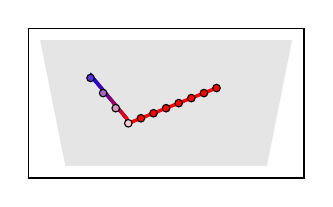
\begin{tikzpicture}[scale=0.32, >=triangle 45, show background rectangle,
  declare function = {
    rotx(\x,\y,\th) = cos(\th)*\x - sin(\th)*\y; % NB! Cannot have space between parameters it seems!
    roty(\x,\y,\th) = sin(\th)*\x + cos(\th)*\y;
  }
  ]

  % View frustum
  \fill[fill=gray!20] (1, 0) -- (9, 0) -- (10, 5) -- (0, 5) -- cycle;


  % Defining some figure params

  \def \pixelwidth  {0.4}
  \def \pixelheight {0.3}
  \def \redstart    {2.2}
  \def \redpixels   {5}
  \def \pixels      {11}
  \def \linewidth   {1.25pt}
  \def \cx          {5}
  \def \cy          {2.5}

  \pgfmathsetmacro\halfpixelwidth{0.5*\pixelwidth}


  \foreach \frame in {0} {  % , ..., 4} {
    \pgfmathsetmacro\theta{25*\frame}

    \ifthenelse{ \frame = 0 \OR \frame = 2 \OR \frame = 4} {
      \def \rightcolToUse {red!100}
      \def \leftcolLToUse {blue!100}
      \def \leftcolRToUse {red!100}
    }{
      \def \rightcolToUse {red!10}
      \def \leftcolLToUse {blue!10}
      \def \leftcolRToUse {red!10}
    }
    
    \def \withSplats {1}
    \def \withLargeSplats {0}
    \def \withConstantWidthSplats {1}
    \def \withFragDepth {0}

        \pgfmathsetmacro\s{1}
    \pgfmathsetmacro\posx{0.5*(\s-1) + 2}
    \pgfmathsetmacro\posy{3.5 - 0.6*(\s-1)}
    \pgfmathsetmacro\posxRot{rotx(\posx-\cx, \posy-\cy, 0)+\cx}
    \pgfmathsetmacro\posyRot{roty(\posx-\cx, \posy-\cy, 0)+\cy}
    \coordinate (left) at ( \posxRot, \posyRot );
    
    \pgfmathsetmacro\s{\redpixels - 1}
    \pgfmathsetmacro\posx{0.5*(\s-1) + 2}
    \pgfmathsetmacro\posy{3.5 - 0.6*(\s-1)}
    \pgfmathsetmacro\posxRot{rotx(\posx-\cx, \posy-\cy, 0)+\cx}
    \pgfmathsetmacro\posyRot{roty(\posx-\cx, \posy-\cy, 0)+\cy}
    \coordinate (middle) at ( \posxRot, \posyRot );
    
    % The offset necessary for the red and green lines to meet properly
    \pgfmathsetmacro\redgreenintersection{3.5 -(0.6+0.2)*(\s-1)}
    
    \pgfmathsetmacro\s{\pixels}
    \pgfmathsetmacro\posx{0.5*(\s-1) + 2}
    \pgfmathsetmacro\posy{0.2*(\s-1) + \redgreenintersection}
    \pgfmathsetmacro\posxRot{rotx(\posx-\cx, \posy-\cy, 0)+\cx}
    \pgfmathsetmacro\posyRot{roty(\posx-\cx, \posy-\cy, 0)+\cy}
    \coordinate (right) at ( \posxRot, \posyRot );
    
    % The "server-rendered model"
    \fill[left color=\leftcolLToUse, right color=\leftcolRToUse, draw=none]
      (left) -- (middle) -- +(0, 5*\linewidth) -- ($ (left) + (0, 5*\linewidth) $) -- cycle;
    % Why is the factor 3 needed here?!?!
    % And why is there a (very thin) border?
    % And why is it not equally thick everywhere?
    \draw[\rightcolToUse, line width=\linewidth] (middle) -- (right);

    \ifthenelse{ \withSplats = 1 } {
      \foreach \s in {1, ..., \pixels} {
        \ifthenelse{\s < \redpixels} {
          \pgfmathsetmacro\posx{0.5*(\s-1) + 2}
          \pgfmathsetmacro\posy{3.5 - 0.6*(\s-1)}
          \pgfmathsetmacro\posxRot{rotx(\posx-\cx, \posy-\cy, \theta)+\cx}
          \pgfmathsetmacro\posyRot{roty(\posx-\cx, \posy-\cy, \theta)+\cy}
          
          % Screen-space-sized splats
          \pgfmathsetmacro\posx{0.5*(\s-1-1) + 2}
          \pgfmathsetmacro\posy{3.5 - 0.6*(\s-1-1)}
          \pgfmathsetmacro\posxRotL{rotx(\posx-\cx, \posy-\cy, \theta)+\cx}
          \pgfmathsetmacro\posyRotL{roty(\posx-\cx, \posy-\cy, \theta)+\cy}
          \pgfmathsetmacro\posx{0.5*(\s-1) + 2}
          \pgfmathsetmacro\posy{3.5 - 0.6*(\s-1)}
          \pgfmathsetmacro\posxRotR{rotx(\posx-\cx, \posy-\cy, \theta)+\cx}
          \pgfmathsetmacro\posyRotR{roty(\posx-\cx, \posy-\cy, \theta)+\cy}
          \pgfmathsetmacro\halfWidthToUse{0.5*(\posxRotR-\posxRotL)}
          
          % Overriding with constant width for one of the sub-figures
          \ifthenelse{ \withConstantWidthSplats = 1 } {
            \pgfmathsetmacro\halfWidthToUse{\halfpixelwidth}
          }{}

          \ifthenelse{ \withLargeSplats = 1 } {
            % Varying color here on the left side
            \pgfmathsetmacro\tl{100*(\s-1)/\redpixels}
            \pgfmathsetmacro\ul{100-\tl)}
            \pgfmathsetmacro\tr{100*(\s  )/\redpixels}
            \pgfmathsetmacro\ur{100-\tr}
            \ifthenelse{ \withFragDepth = 0 } {
              \draw[left color=red!\tl!blue!\ul, right color=red!\tr!blue!\ur]
                (\posxRot-\halfWidthToUse, \posyRot) rectangle +(2*\halfWidthToUse, 0.2);
            }{
              % Tror kanskje at problemet med at ting kommer for langt til venstre her, skyldes at vi ser paa 
              % linjestykker fra s-1-1 til s-1. Burde muligens vaert fra s-1-0.5 til s-1+0.5?!
              % Replace with rotated rectangles, will probably look better...
              \draw[left color=red!\tl!blue!\ul, right color=red!\tr!blue!\ur]
                (\posxRotL, \posyRotL) -- (\posxRotR, \posyRotR) -- +(0, 5*\linewidth) -- 
                ($ (\posxRotL, \posyRotL) + (0, 5*\linewidth) $) -- cycle;
            }
          }{
            % Constant color, just a dot
            \pgfmathsetmacro\t{100*\s/\redpixels}
            \pgfmathsetmacro\u{100*(1.0-\s/\redpixels)}
            \draw[fill=red!\t!blue!\u] (\posxRot, \posyRot) circle(0.15);
          }
        } {
          \pgfmathsetmacro\posx{0.5*(\s-1) + 2}
          \pgfmathsetmacro\posy{0.2*(\s-1) + \redgreenintersection}
          \pgfmathsetmacro\posxRot{rotx(\posx-\cx, \posy-\cy, \theta)+\cx}
          \pgfmathsetmacro\posyRot{roty(\posx-\cx, \posy-\cy, \theta)+\cy}
          
          % Screen-space-sized splats
          \pgfmathsetmacro\posx{0.5*(\s-1-1) + 2}
          \pgfmathsetmacro\posy{0.2*(\s-1-1) + \redgreenintersection}
          \pgfmathsetmacro\posxRotL{rotx(\posx-\cx, \posy-\cy, \theta)+\cx}
          \pgfmathsetmacro\posyRotL{roty(\posx-\cx, \posy-\cy, \theta)+\cy}
          \pgfmathsetmacro\posx{0.5*(\s-1) + 2}
          \pgfmathsetmacro\posy{0.2*(\s-1) + \redgreenintersection}
          \pgfmathsetmacro\posxRotR{rotx(\posx-\cx, \posy-\cy, \theta)+\cx}
          \pgfmathsetmacro\posyRotR{roty(\posx-\cx, \posy-\cy, \theta)+\cy}
          \pgfmathsetmacro\halfWidthToUse{0.5*(\posxRotR-\posxRotL)}
          
          \ifthenelse{ \withConstantWidthSplats = 1 } {
            % Overriding with constant width for one of the sub-figures
            \pgfmathsetmacro\halfWidthToUse{\halfpixelwidth}
          }{}

          \ifthenelse{ \withLargeSplats = 1 } {
            \ifthenelse{ \withFragDepth = 0 } {
              \draw[fill=\rightcolToUse]
                (\posxRot-\halfWidthToUse, \posyRot) rectangle +(2*\halfWidthToUse, 0.2);
            }{
              % \draw[fill=\rightcolToUse, line width=1.5pt] (\posxRotL, \posyRotL) -- (\posxRotR, \posyRotR);
              % Tror kanskje at problemet med at ting kommer for langt til venstre her, skyldes at vi ser paa 
              % linjestykker fra s-1-1 til s-1. Burde muligens vaert fra s-1-0.5 til s-1+0.5?!
              % Replace with rotated rectangles, will probably look better...
              \draw[fill=\rightcolToUse]
                (\posxRotL, \posyRotL) -- (\posxRotR, \posyRotR) -- +(0, 5*\linewidth) -- 
                ($ (\posxRotL, \posyRotL) + (0, 5*\linewidth) $) -- cycle;
            }
          }{
            % Constant color, just a dot
            \draw[fill=\rightcolToUse] (\posxRot, \posyRot) circle(0.15);
          }
        }
      }
    }{}

    
  }


\end{tikzpicture}

  }
  \subfigure[Client-generated frame]{
    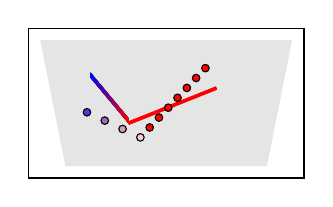
\begin{tikzpicture}[scale=0.32, >=triangle 45, show background rectangle,
  declare function = {
    rotx(\x,\y,\th) = cos(\th)*\x - sin(\th)*\y; % NB! Cannot have space between parameters it seems!
    roty(\x,\y,\th) = sin(\th)*\x + cos(\th)*\y;
  }
  ]

  % View frustum
  \fill[fill=gray!20] (1, 0) -- (9, 0) -- (10, 5) -- (0, 5) -- cycle;


  % Defining some figure params

  \def \pixelwidth  {0.5}
  \def \pixelheight {0.3}
  \def \redstart    {2.2}
  \def \redpixels   {5}
  \def \pixels      {11}
  \def \linewidth   {1.25pt}
  \def \theta       {25}        % Degrees
  \def \cx          {5}
  \def \cy          {2.5}

  \pgfmathsetmacro\halfpixelwidth{0.5*\pixelwidth}


  \foreach \frame in {0, ..., 1} {  % , ..., 4} {
    \pgfmathsetmacro\theta{25*\frame}

    \def \rightcolToUse {red!100}
    \def \leftcolLToUse {blue!100}
    \def \leftcolRToUse {red!100}

    \ifthenelse{ \frame = 0 } {
      \def \withSplats {0}
    }{
      \def \withSplats {1}
    }
    \def \withLargeSplats {0}
    \def \withConstantWidthSplats {1}
    \def \withFragDepth {0}

        \pgfmathsetmacro\s{1}
    \pgfmathsetmacro\posx{0.5*(\s-1) + 2}
    \pgfmathsetmacro\posy{3.5 - 0.6*(\s-1)}
    \pgfmathsetmacro\posxRot{rotx(\posx-\cx, \posy-\cy, 0)+\cx}
    \pgfmathsetmacro\posyRot{roty(\posx-\cx, \posy-\cy, 0)+\cy}
    \coordinate (left) at ( \posxRot, \posyRot );
    
    \pgfmathsetmacro\s{\redpixels - 1}
    \pgfmathsetmacro\posx{0.5*(\s-1) + 2}
    \pgfmathsetmacro\posy{3.5 - 0.6*(\s-1)}
    \pgfmathsetmacro\posxRot{rotx(\posx-\cx, \posy-\cy, 0)+\cx}
    \pgfmathsetmacro\posyRot{roty(\posx-\cx, \posy-\cy, 0)+\cy}
    \coordinate (middle) at ( \posxRot, \posyRot );
    
    % The offset necessary for the red and green lines to meet properly
    \pgfmathsetmacro\redgreenintersection{3.5 -(0.6+0.2)*(\s-1)}
    
    \pgfmathsetmacro\s{\pixels}
    \pgfmathsetmacro\posx{0.5*(\s-1) + 2}
    \pgfmathsetmacro\posy{0.2*(\s-1) + \redgreenintersection}
    \pgfmathsetmacro\posxRot{rotx(\posx-\cx, \posy-\cy, 0)+\cx}
    \pgfmathsetmacro\posyRot{roty(\posx-\cx, \posy-\cy, 0)+\cy}
    \coordinate (right) at ( \posxRot, \posyRot );
    
    % The "server-rendered model"
    \fill[left color=\leftcolLToUse, right color=\leftcolRToUse, draw=none]
      (left) -- (middle) -- +(0, 5*\linewidth) -- ($ (left) + (0, 5*\linewidth) $) -- cycle;
    % Why is the factor 3 needed here?!?!
    % And why is there a (very thin) border?
    % And why is it not equally thick everywhere?
    \draw[\rightcolToUse, line width=\linewidth] (middle) -- (right);

    \ifthenelse{ \withSplats = 1 } {
      \foreach \s in {1, ..., \pixels} {
        \ifthenelse{\s < \redpixels} {
          \pgfmathsetmacro\posx{0.5*(\s-1) + 2}
          \pgfmathsetmacro\posy{3.5 - 0.6*(\s-1)}
          \pgfmathsetmacro\posxRot{rotx(\posx-\cx, \posy-\cy, \theta)+\cx}
          \pgfmathsetmacro\posyRot{roty(\posx-\cx, \posy-\cy, \theta)+\cy}
          
          % Screen-space-sized splats
          \pgfmathsetmacro\posx{0.5*(\s-1-1) + 2}
          \pgfmathsetmacro\posy{3.5 - 0.6*(\s-1-1)}
          \pgfmathsetmacro\posxRotL{rotx(\posx-\cx, \posy-\cy, \theta)+\cx}
          \pgfmathsetmacro\posyRotL{roty(\posx-\cx, \posy-\cy, \theta)+\cy}
          \pgfmathsetmacro\posx{0.5*(\s-1) + 2}
          \pgfmathsetmacro\posy{3.5 - 0.6*(\s-1)}
          \pgfmathsetmacro\posxRotR{rotx(\posx-\cx, \posy-\cy, \theta)+\cx}
          \pgfmathsetmacro\posyRotR{roty(\posx-\cx, \posy-\cy, \theta)+\cy}
          \pgfmathsetmacro\halfWidthToUse{0.5*(\posxRotR-\posxRotL)}
          
          % Overriding with constant width for one of the sub-figures
          \ifthenelse{ \withConstantWidthSplats = 1 } {
            \pgfmathsetmacro\halfWidthToUse{\halfpixelwidth}
          }{}

          \ifthenelse{ \withLargeSplats = 1 } {
            % Varying color here on the left side
            \pgfmathsetmacro\tl{100*(\s-1)/\redpixels}
            \pgfmathsetmacro\ul{100-\tl)}
            \pgfmathsetmacro\tr{100*(\s  )/\redpixels}
            \pgfmathsetmacro\ur{100-\tr}
            \ifthenelse{ \withFragDepth = 0 } {
              \draw[left color=red!\tl!blue!\ul, right color=red!\tr!blue!\ur]
                (\posxRot-\halfWidthToUse, \posyRot) rectangle +(2*\halfWidthToUse, 0.2);
            }{
              % Tror kanskje at problemet med at ting kommer for langt til venstre her, skyldes at vi ser paa 
              % linjestykker fra s-1-1 til s-1. Burde muligens vaert fra s-1-0.5 til s-1+0.5?!
              % Replace with rotated rectangles, will probably look better...
              \draw[left color=red!\tl!blue!\ul, right color=red!\tr!blue!\ur]
                (\posxRotL, \posyRotL) -- (\posxRotR, \posyRotR) -- +(0, 5*\linewidth) -- 
                ($ (\posxRotL, \posyRotL) + (0, 5*\linewidth) $) -- cycle;
            }
          }{
            % Constant color, just a dot
            \pgfmathsetmacro\t{100*\s/\redpixels}
            \pgfmathsetmacro\u{100*(1.0-\s/\redpixels)}
            \draw[fill=red!\t!blue!\u] (\posxRot, \posyRot) circle(0.15);
          }
        } {
          \pgfmathsetmacro\posx{0.5*(\s-1) + 2}
          \pgfmathsetmacro\posy{0.2*(\s-1) + \redgreenintersection}
          \pgfmathsetmacro\posxRot{rotx(\posx-\cx, \posy-\cy, \theta)+\cx}
          \pgfmathsetmacro\posyRot{roty(\posx-\cx, \posy-\cy, \theta)+\cy}
          
          % Screen-space-sized splats
          \pgfmathsetmacro\posx{0.5*(\s-1-1) + 2}
          \pgfmathsetmacro\posy{0.2*(\s-1-1) + \redgreenintersection}
          \pgfmathsetmacro\posxRotL{rotx(\posx-\cx, \posy-\cy, \theta)+\cx}
          \pgfmathsetmacro\posyRotL{roty(\posx-\cx, \posy-\cy, \theta)+\cy}
          \pgfmathsetmacro\posx{0.5*(\s-1) + 2}
          \pgfmathsetmacro\posy{0.2*(\s-1) + \redgreenintersection}
          \pgfmathsetmacro\posxRotR{rotx(\posx-\cx, \posy-\cy, \theta)+\cx}
          \pgfmathsetmacro\posyRotR{roty(\posx-\cx, \posy-\cy, \theta)+\cy}
          \pgfmathsetmacro\halfWidthToUse{0.5*(\posxRotR-\posxRotL)}
          
          \ifthenelse{ \withConstantWidthSplats = 1 } {
            % Overriding with constant width for one of the sub-figures
            \pgfmathsetmacro\halfWidthToUse{\halfpixelwidth}
          }{}

          \ifthenelse{ \withLargeSplats = 1 } {
            \ifthenelse{ \withFragDepth = 0 } {
              \draw[fill=\rightcolToUse]
                (\posxRot-\halfWidthToUse, \posyRot) rectangle +(2*\halfWidthToUse, 0.2);
            }{
              % \draw[fill=\rightcolToUse, line width=1.5pt] (\posxRotL, \posyRotL) -- (\posxRotR, \posyRotR);
              % Tror kanskje at problemet med at ting kommer for langt til venstre her, skyldes at vi ser paa 
              % linjestykker fra s-1-1 til s-1. Burde muligens vaert fra s-1-0.5 til s-1+0.5?!
              % Replace with rotated rectangles, will probably look better...
              \draw[fill=\rightcolToUse]
                (\posxRotL, \posyRotL) -- (\posxRotR, \posyRotR) -- +(0, 5*\linewidth) -- 
                ($ (\posxRotL, \posyRotL) + (0, 5*\linewidth) $) -- cycle;
            }
          }{
            % Constant color, just a dot
            \draw[fill=\rightcolToUse] (\posxRot, \posyRot) circle(0.15);
          }
        }
      }
    }{}

    
  }
  

\end{tikzpicture}

  }
  \subfigure[With texturing]{
    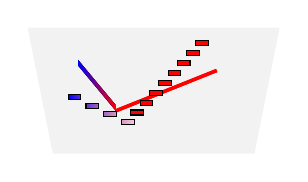
\begin{tikzpicture}[scale=0.32, >=triangle 45, % show background rectangle,
  declare function = {
    rotx(\x,\y,\th) = cos(\th)*\x - sin(\th)*\y; % NB! Cannot have space between parameters it seems!
    roty(\x,\y,\th) = sin(\th)*\x + cos(\th)*\y;
  }
  ]

  % View frustum
\fill[fill=gray!10] (1, 0) -- (9, 0) -- (10, 5) -- (0, 5) -- cycle;

% \clip (1, 0) -- (9, 0) -- (10, 5) -- (0, 5) -- cycle;

% Clipping looks ok, but clipped content still expands bbox!! Solving this by
% reducing \pixels below from 13 to 11...


% Defining some figure params

\def \pixelwidth  {0.5}
\def \pixelheight {0.3}
\def \theta       {25}        % Degrees
%\def \pixelwidth  {0.4}
%\def \pixelheight {0.3}
\def \redstart    {2.2}
\def \redpixels   {5}
\def \pixels      {12}
\def \linewidth   {1.25pt}
\def \cx          {5}
\def \cy          {2.5}

% bare for fig3a.tex: ?
\def \rightcol    {red!100}
\def \leftcolL    {blue!100}
%\def \leftcolR    {red!100!blue!0} % Why doesn't this work?! (The color becomes white)
\def \leftcolR    {red!100}

\pgfmathsetmacro\halfpixelwidth{0.5*\pixelwidth}


  \foreach \frame in {0, ..., 1} {
    \pgfmathsetmacro\theta{25*\frame}

    \def \rightcolToUse {red!100}
    \def \leftcolLToUse {blue!100}
    \def \leftcolRToUse {red!100}

    \ifthenelse{ \frame = 0 } {
      \def \withSplats {0}
    }{
      \def \withSplats {1}
    }
    \def \withLargeSplats {1}
    \def \withConstantWidthSplats {1}
    \def \withFragDepth {0}

        \pgfmathsetmacro\s{1}
    \pgfmathsetmacro\posx{0.5*(\s-1) + 2}
    \pgfmathsetmacro\posy{3.5 - 0.6*(\s-1)}
    \pgfmathsetmacro\posxRot{rotx(\posx-\cx, \posy-\cy, 0)+\cx}
    \pgfmathsetmacro\posyRot{roty(\posx-\cx, \posy-\cy, 0)+\cy}
    \coordinate (left) at ( \posxRot, \posyRot );
    
    \pgfmathsetmacro\s{\redpixels - 1}
    \pgfmathsetmacro\posx{0.5*(\s-1) + 2}
    \pgfmathsetmacro\posy{3.5 - 0.6*(\s-1)}
    \pgfmathsetmacro\posxRot{rotx(\posx-\cx, \posy-\cy, 0)+\cx}
    \pgfmathsetmacro\posyRot{roty(\posx-\cx, \posy-\cy, 0)+\cy}
    \coordinate (middle) at ( \posxRot, \posyRot );
    
    % The offset necessary for the red and green lines to meet properly
    \pgfmathsetmacro\redgreenintersection{3.5 -(0.6+0.2)*(\s-1)}
    
    \pgfmathsetmacro\s{\pixels}
    \pgfmathsetmacro\posx{0.5*(\s-1) + 2}
    \pgfmathsetmacro\posy{0.2*(\s-1) + \redgreenintersection}
    \pgfmathsetmacro\posxRot{rotx(\posx-\cx, \posy-\cy, 0)+\cx}
    \pgfmathsetmacro\posyRot{roty(\posx-\cx, \posy-\cy, 0)+\cy}
    \coordinate (right) at ( \posxRot, \posyRot );
    
    % The "server-rendered model"
    \fill[left color=\leftcolLToUse, right color=\leftcolRToUse, draw=none]
      (left) -- (middle) -- +(0, 5*\linewidth) -- ($ (left) + (0, 5*\linewidth) $) -- cycle;
    % Why is the factor 3 needed here?!?!
    % And why is there a (very thin) border?
    % And why is it not equally thick everywhere?
    \draw[\rightcolToUse, line width=\linewidth] (middle) -- (right);

    \ifthenelse{ \withSplats = 1 } {
      \foreach \s in {1, ..., \pixels} {
        \ifthenelse{\s < \redpixels} {
          \pgfmathsetmacro\posx{0.5*(\s-1) + 2}
          \pgfmathsetmacro\posy{3.5 - 0.6*(\s-1)}
          \pgfmathsetmacro\posxRot{rotx(\posx-\cx, \posy-\cy, \theta)+\cx}
          \pgfmathsetmacro\posyRot{roty(\posx-\cx, \posy-\cy, \theta)+\cy}
          
          % Screen-space-sized splats
          \pgfmathsetmacro\posx{0.5*(\s-1-1) + 2}
          \pgfmathsetmacro\posy{3.5 - 0.6*(\s-1-1)}
          \pgfmathsetmacro\posxRotL{rotx(\posx-\cx, \posy-\cy, \theta)+\cx}
          \pgfmathsetmacro\posyRotL{roty(\posx-\cx, \posy-\cy, \theta)+\cy}
          \pgfmathsetmacro\posx{0.5*(\s-1) + 2}
          \pgfmathsetmacro\posy{3.5 - 0.6*(\s-1)}
          \pgfmathsetmacro\posxRotR{rotx(\posx-\cx, \posy-\cy, \theta)+\cx}
          \pgfmathsetmacro\posyRotR{roty(\posx-\cx, \posy-\cy, \theta)+\cy}
          \pgfmathsetmacro\halfWidthToUse{0.5*(\posxRotR-\posxRotL)}
          
          % Overriding with constant width for one of the sub-figures
          \ifthenelse{ \withConstantWidthSplats = 1 } {
            \pgfmathsetmacro\halfWidthToUse{\halfpixelwidth}
          }{}

          \ifthenelse{ \withLargeSplats = 1 } {
            % Varying color here on the left side
            \pgfmathsetmacro\tl{100*(\s-1)/\redpixels}
            \pgfmathsetmacro\ul{100-\tl)}
            \pgfmathsetmacro\tr{100*(\s  )/\redpixels}
            \pgfmathsetmacro\ur{100-\tr}
            \ifthenelse{ \withFragDepth = 0 } {
              \draw[left color=red!\tl!blue!\ul, right color=red!\tr!blue!\ur]
                (\posxRot-\halfWidthToUse, \posyRot) rectangle +(2*\halfWidthToUse, 0.2);
            }{
              % Tror kanskje at problemet med at ting kommer for langt til venstre her, skyldes at vi ser paa 
              % linjestykker fra s-1-1 til s-1. Burde muligens vaert fra s-1-0.5 til s-1+0.5?!
              % Replace with rotated rectangles, will probably look better...
              \draw[left color=red!\tl!blue!\ul, right color=red!\tr!blue!\ur]
                (\posxRotL, \posyRotL) -- (\posxRotR, \posyRotR) -- +(0, 5*\linewidth) -- 
                ($ (\posxRotL, \posyRotL) + (0, 5*\linewidth) $) -- cycle;
            }
          }{
            % Constant color, just a dot
            \pgfmathsetmacro\t{100*\s/\redpixels}
            \pgfmathsetmacro\u{100*(1.0-\s/\redpixels)}
            \draw[fill=red!\t!blue!\u] (\posxRot, \posyRot) circle(0.15);
          }
        } {
          \pgfmathsetmacro\posx{0.5*(\s-1) + 2}
          \pgfmathsetmacro\posy{0.2*(\s-1) + \redgreenintersection}
          \pgfmathsetmacro\posxRot{rotx(\posx-\cx, \posy-\cy, \theta)+\cx}
          \pgfmathsetmacro\posyRot{roty(\posx-\cx, \posy-\cy, \theta)+\cy}
          
          % Screen-space-sized splats
          \pgfmathsetmacro\posx{0.5*(\s-1-1) + 2}
          \pgfmathsetmacro\posy{0.2*(\s-1-1) + \redgreenintersection}
          \pgfmathsetmacro\posxRotL{rotx(\posx-\cx, \posy-\cy, \theta)+\cx}
          \pgfmathsetmacro\posyRotL{roty(\posx-\cx, \posy-\cy, \theta)+\cy}
          \pgfmathsetmacro\posx{0.5*(\s-1) + 2}
          \pgfmathsetmacro\posy{0.2*(\s-1) + \redgreenintersection}
          \pgfmathsetmacro\posxRotR{rotx(\posx-\cx, \posy-\cy, \theta)+\cx}
          \pgfmathsetmacro\posyRotR{roty(\posx-\cx, \posy-\cy, \theta)+\cy}
          \pgfmathsetmacro\halfWidthToUse{0.5*(\posxRotR-\posxRotL)}
          
          \ifthenelse{ \withConstantWidthSplats = 1 } {
            % Overriding with constant width for one of the sub-figures
            \pgfmathsetmacro\halfWidthToUse{\halfpixelwidth}
          }{}

          \ifthenelse{ \withLargeSplats = 1 } {
            \ifthenelse{ \withFragDepth = 0 } {
              \draw[fill=\rightcolToUse]
                (\posxRot-\halfWidthToUse, \posyRot) rectangle +(2*\halfWidthToUse, 0.2);
            }{
              % \draw[fill=\rightcolToUse, line width=1.5pt] (\posxRotL, \posyRotL) -- (\posxRotR, \posyRotR);
              % Tror kanskje at problemet med at ting kommer for langt til venstre her, skyldes at vi ser paa 
              % linjestykker fra s-1-1 til s-1. Burde muligens vaert fra s-1-0.5 til s-1+0.5?!
              % Replace with rotated rectangles, will probably look better...
              \draw[fill=\rightcolToUse]
                (\posxRotL, \posyRotL) -- (\posxRotR, \posyRotR) -- +(0, 5*\linewidth) -- 
                ($ (\posxRotL, \posyRotL) + (0, 5*\linewidth) $) -- cycle;
            }
          }{
            % Constant color, just a dot
            \draw[fill=\rightcolToUse] (\posxRot, \posyRot) circle(0.15);
          }
        }
      }
    }{}

    
  }


\end{tikzpicture}

  }
  \subfigure[Screen-space-sized splats]{
    %\begin{tikzpicture}[ scale=.25, show background rectangle]
\begin{tikzpicture}[scale=0.32, >=triangle 45, show background rectangle,
  declare function = {
    rotx(\x,\y,\th) = cos(\th)*\x - sin(\th)*\y; % NB! Cannot have space between parameters it seems!
    roty(\x,\y,\th) = sin(\th)*\x + cos(\th)*\y;
  }
  ]

  % View frustum
  \fill[fill=gray!20] (1, 0) -- (9, 0) -- (10, 5) -- (0, 5) -- cycle;


  % Defining some figure params

  \def \pixelwidth  {0.5}
  \def \pixelheight {0.3}
  \def \redstart    {2.2}
  \def \redpixels   {5}
  \def \pixels      {13}
  \def \linewidth   {1.25pt}
  \def \theta       {25}        % Degrees
  \def \cx          {5}
  \def \cy          {2.5}

  \pgfmathsetmacro\halfpixelwidth{0.5*\pixelwidth}


  % The scene, using same coordinate calculations as in the loop below

  \pgfmathsetmacro\s{1}
  \pgfmathsetmacro\posx{0.5*(\s-1) + 2}
  \pgfmathsetmacro\posy{3.5 - 0.6*(\s-1)}
  \pgfmathsetmacro\posxRot{rotx(\posx-\cx, \posy-\cy, 0)+\cx}
  \pgfmathsetmacro\posyRot{roty(\posx-\cx, \posy-\cy, 0)+\cy}
  \coordinate (left) at ( \posxRot, \posyRot );

  \pgfmathsetmacro\s{\redpixels - 1}
  \pgfmathsetmacro\posx{0.5*(\s-1) + 2}
  \pgfmathsetmacro\posy{3.5 - 0.6*(\s-1)}
  \pgfmathsetmacro\posxRot{rotx(\posx-\cx, \posy-\cy, 0)+\cx}
  \pgfmathsetmacro\posyRot{roty(\posx-\cx, \posy-\cy, 0)+\cy}
  \coordinate (middle) at ( \posxRot, \posyRot );

  % The offset necessary for the red and green lines to meet properly
  \pgfmathsetmacro\redgreenintersection{3.5 -(0.6+0.2)*(\s-1)}

  \pgfmathsetmacro\s{\pixels}
  \pgfmathsetmacro\posx{0.5*(\s-1) + 2}
  \pgfmathsetmacro\posy{0.2*(\s-1) + \redgreenintersection}
  \pgfmathsetmacro\posxRot{rotx(\posx-\cx, \posy-\cy, 0)+\cx}
  \pgfmathsetmacro\posyRot{roty(\posx-\cx, \posy-\cy, 0)+\cy}
  \coordinate (right) at ( \posxRot, \posyRot );

  \draw[red!50, line width=\linewidth] (left) -- (middle);
  \draw[green!50, line width=\linewidth] (middle) -- (right);


  % Showing splats

  \foreach \s in {1, ..., \pixels} {
    \ifthenelse{\s < \redpixels} {
      \pgfmathsetmacro\posx{0.5*(\s-1) + 2}
      \pgfmathsetmacro\posy{3.5 - 0.6*(\s-1)}
      \pgfmathsetmacro\posxRot{rotx(\posx-\cx, \posy-\cy, \theta)+\cx}
      \pgfmathsetmacro\posyRot{roty(\posx-\cx, \posy-\cy, \theta)+\cy}

      % Screen-space-sized splats
      \pgfmathsetmacro\posx{0.5*(\s-1-1) + 2}
      \pgfmathsetmacro\posy{3.5 - 0.6*(\s-1-1)}
      \pgfmathsetmacro\posxRotL{rotx(\posx-\cx, \posy-\cy, \theta)+\cx}
      \pgfmathsetmacro\posx{0.5*(\s-1) + 2}
      \pgfmathsetmacro\posy{3.5 - 0.6*(\s-1)}
      \pgfmathsetmacro\posxRotR{rotx(\posx-\cx, \posy-\cy, \theta)+\cx}
      \pgfmathsetmacro\halfWidthToUse{0.5*(\posxRotR-\posxRotL)}

      %\pgfmathsetmacro\halfWidthToUse{\halfpixelwidth}

%      \draw[red, fill=red!50, line width=1.5pt] (\posxRot, \posyRot) -- +(-\halfWidthToUse, 0);
%      \draw[red, fill=red!50, line width=1.5pt] (\posxRot, \posyRot) -- +(\halfWidthToUse, 0);

      % Varying color
      \pgfmathsetmacro\tl{100*(\s-1)/\redpixels}
      \pgfmathsetmacro\ul{100-\tl)}
      \pgfmathsetmacro\tr{100*(\s  )/\redpixels}
      \pgfmathsetmacro\ur{100-\tr}
      \shade[left color=red!\tl!blue!\ul, right color=red!\tr!blue!\ur, line width=1.5pt] (\posxRot-\halfWidthToUse, \posyRot) rectangle +(2*\halfWidthToUse, 0.2);

      %\draw[red, fill=red!50] (\posxRot, \posyRot) circle(0.15);
    } {
      \pgfmathsetmacro\posx{0.5*(\s-1) + 2}
      \pgfmathsetmacro\posy{0.2*(\s-1) + \redgreenintersection}
      \pgfmathsetmacro\posxRot{rotx(\posx-\cx, \posy-\cy, \theta)+\cx}
      \pgfmathsetmacro\posyRot{roty(\posx-\cx, \posy-\cy, \theta)+\cy}

      % Screen-space-sized splats
      \pgfmathsetmacro\posx{0.5*(\s-1-1) + 2}
      \pgfmathsetmacro\posy{0.2*(\s-1-1) + \redgreenintersection}
      \pgfmathsetmacro\posxRotL{rotx(\posx-\cx, \posy-\cy, \theta)+\cx}
      \pgfmathsetmacro\posx{0.5*(\s-1) + 2}
      \pgfmathsetmacro\posy{0.2*(\s-1) + \redgreenintersection}
      \pgfmathsetmacro\posxRotR{rotx(\posx-\cx, \posy-\cy, \theta)+\cx}
      \pgfmathsetmacro\halfWidthToUse{0.5*(\posxRotR-\posxRotL)}

      %\pgfmathsetmacro\halfWidthToUse{\halfpixelwidth}

      \draw[green, fill=green!50, line width=1.5pt] (\posxRot, \posyRot) -- +(-\halfWidthToUse, 0);
      \draw[green, fill=green!50, line width=1.5pt] (\posxRot, \posyRot) -- +(\halfWidthToUse, 0);

      %\draw[green, fill=green!50] (\posxRot, \posyRot) circle(0.15);
    }
  }


\end{tikzpicture}

  }
  \subfigure[With intra-splat depths]{
    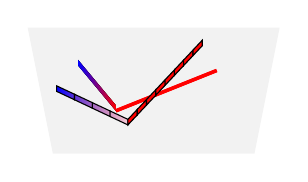
\begin{tikzpicture}[scale=0.32, >=triangle 45, % show background rectangle,
  declare function = {
    rotx(\x,\y,\th) = cos(\th)*\x - sin(\th)*\y; % NB! Cannot have space between parameters it seems!
    roty(\x,\y,\th) = sin(\th)*\x + cos(\th)*\y;
  }
  ]

  % View frustum
\fill[fill=gray!10] (1, 0) -- (9, 0) -- (10, 5) -- (0, 5) -- cycle;

% \clip (1, 0) -- (9, 0) -- (10, 5) -- (0, 5) -- cycle;

% Clipping looks ok, but clipped content still expands bbox!! Solving this by
% reducing \pixels below from 13 to 11...


% Defining some figure params

\def \pixelwidth  {0.5}
\def \pixelheight {0.3}
\def \theta       {25}        % Degrees
%\def \pixelwidth  {0.4}
%\def \pixelheight {0.3}
\def \redstart    {2.2}
\def \redpixels   {5}
\def \pixels      {12}
\def \linewidth   {1.25pt}
\def \cx          {5}
\def \cy          {2.5}

% bare for fig3a.tex: ?
\def \rightcol    {red!100}
\def \leftcolL    {blue!100}
%\def \leftcolR    {red!100!blue!0} % Why doesn't this work?! (The color becomes white)
\def \leftcolR    {red!100}

\pgfmathsetmacro\halfpixelwidth{0.5*\pixelwidth}


  \foreach \frame in {0, ..., 1} {
    \pgfmathsetmacro\theta{25*\frame}

    \def \rightcolToUse {red!100}
    \def \leftcolLToUse {blue!100}
    \def \leftcolRToUse {red!100}

    \ifthenelse{ \frame = 0 } {
      \def \withSplats {0}
    }{
      \def \withSplats {1}
    }
    \def \withLargeSplats {1}
    \def \withConstantWidthSplats {0}
    \def \withFragDepth {1}

        \pgfmathsetmacro\s{1}
    \pgfmathsetmacro\posx{0.5*(\s-1) + 2}
    \pgfmathsetmacro\posy{3.5 - 0.6*(\s-1)}
    \pgfmathsetmacro\posxRot{rotx(\posx-\cx, \posy-\cy, 0)+\cx}
    \pgfmathsetmacro\posyRot{roty(\posx-\cx, \posy-\cy, 0)+\cy}
    \coordinate (left) at ( \posxRot, \posyRot );
    
    \pgfmathsetmacro\s{\redpixels - 1}
    \pgfmathsetmacro\posx{0.5*(\s-1) + 2}
    \pgfmathsetmacro\posy{3.5 - 0.6*(\s-1)}
    \pgfmathsetmacro\posxRot{rotx(\posx-\cx, \posy-\cy, 0)+\cx}
    \pgfmathsetmacro\posyRot{roty(\posx-\cx, \posy-\cy, 0)+\cy}
    \coordinate (middle) at ( \posxRot, \posyRot );
    
    % The offset necessary for the red and green lines to meet properly
    \pgfmathsetmacro\redgreenintersection{3.5 -(0.6+0.2)*(\s-1)}
    
    \pgfmathsetmacro\s{\pixels}
    \pgfmathsetmacro\posx{0.5*(\s-1) + 2}
    \pgfmathsetmacro\posy{0.2*(\s-1) + \redgreenintersection}
    \pgfmathsetmacro\posxRot{rotx(\posx-\cx, \posy-\cy, 0)+\cx}
    \pgfmathsetmacro\posyRot{roty(\posx-\cx, \posy-\cy, 0)+\cy}
    \coordinate (right) at ( \posxRot, \posyRot );
    
    % The "server-rendered model"
    \fill[left color=\leftcolLToUse, right color=\leftcolRToUse, draw=none]
      (left) -- (middle) -- +(0, 5*\linewidth) -- ($ (left) + (0, 5*\linewidth) $) -- cycle;
    % Why is the factor 3 needed here?!?!
    % And why is there a (very thin) border?
    % And why is it not equally thick everywhere?
    \draw[\rightcolToUse, line width=\linewidth] (middle) -- (right);

    \ifthenelse{ \withSplats = 1 } {
      \foreach \s in {1, ..., \pixels} {
        \ifthenelse{\s < \redpixels} {
          \pgfmathsetmacro\posx{0.5*(\s-1) + 2}
          \pgfmathsetmacro\posy{3.5 - 0.6*(\s-1)}
          \pgfmathsetmacro\posxRot{rotx(\posx-\cx, \posy-\cy, \theta)+\cx}
          \pgfmathsetmacro\posyRot{roty(\posx-\cx, \posy-\cy, \theta)+\cy}
          
          % Screen-space-sized splats
          \pgfmathsetmacro\posx{0.5*(\s-1-1) + 2}
          \pgfmathsetmacro\posy{3.5 - 0.6*(\s-1-1)}
          \pgfmathsetmacro\posxRotL{rotx(\posx-\cx, \posy-\cy, \theta)+\cx}
          \pgfmathsetmacro\posyRotL{roty(\posx-\cx, \posy-\cy, \theta)+\cy}
          \pgfmathsetmacro\posx{0.5*(\s-1) + 2}
          \pgfmathsetmacro\posy{3.5 - 0.6*(\s-1)}
          \pgfmathsetmacro\posxRotR{rotx(\posx-\cx, \posy-\cy, \theta)+\cx}
          \pgfmathsetmacro\posyRotR{roty(\posx-\cx, \posy-\cy, \theta)+\cy}
          \pgfmathsetmacro\halfWidthToUse{0.5*(\posxRotR-\posxRotL)}
          
          % Overriding with constant width for one of the sub-figures
          \ifthenelse{ \withConstantWidthSplats = 1 } {
            \pgfmathsetmacro\halfWidthToUse{\halfpixelwidth}
          }{}

          \ifthenelse{ \withLargeSplats = 1 } {
            % Varying color here on the left side
            \pgfmathsetmacro\tl{100*(\s-1)/\redpixels}
            \pgfmathsetmacro\ul{100-\tl)}
            \pgfmathsetmacro\tr{100*(\s  )/\redpixels}
            \pgfmathsetmacro\ur{100-\tr}
            \ifthenelse{ \withFragDepth = 0 } {
              \draw[left color=red!\tl!blue!\ul, right color=red!\tr!blue!\ur]
                (\posxRot-\halfWidthToUse, \posyRot) rectangle +(2*\halfWidthToUse, 0.2);
            }{
              % Tror kanskje at problemet med at ting kommer for langt til venstre her, skyldes at vi ser paa 
              % linjestykker fra s-1-1 til s-1. Burde muligens vaert fra s-1-0.5 til s-1+0.5?!
              % Replace with rotated rectangles, will probably look better...
              \draw[left color=red!\tl!blue!\ul, right color=red!\tr!blue!\ur]
                (\posxRotL, \posyRotL) -- (\posxRotR, \posyRotR) -- +(0, 5*\linewidth) -- 
                ($ (\posxRotL, \posyRotL) + (0, 5*\linewidth) $) -- cycle;
            }
          }{
            % Constant color, just a dot
            \pgfmathsetmacro\t{100*\s/\redpixels}
            \pgfmathsetmacro\u{100*(1.0-\s/\redpixels)}
            \draw[fill=red!\t!blue!\u] (\posxRot, \posyRot) circle(0.15);
          }
        } {
          \pgfmathsetmacro\posx{0.5*(\s-1) + 2}
          \pgfmathsetmacro\posy{0.2*(\s-1) + \redgreenintersection}
          \pgfmathsetmacro\posxRot{rotx(\posx-\cx, \posy-\cy, \theta)+\cx}
          \pgfmathsetmacro\posyRot{roty(\posx-\cx, \posy-\cy, \theta)+\cy}
          
          % Screen-space-sized splats
          \pgfmathsetmacro\posx{0.5*(\s-1-1) + 2}
          \pgfmathsetmacro\posy{0.2*(\s-1-1) + \redgreenintersection}
          \pgfmathsetmacro\posxRotL{rotx(\posx-\cx, \posy-\cy, \theta)+\cx}
          \pgfmathsetmacro\posyRotL{roty(\posx-\cx, \posy-\cy, \theta)+\cy}
          \pgfmathsetmacro\posx{0.5*(\s-1) + 2}
          \pgfmathsetmacro\posy{0.2*(\s-1) + \redgreenintersection}
          \pgfmathsetmacro\posxRotR{rotx(\posx-\cx, \posy-\cy, \theta)+\cx}
          \pgfmathsetmacro\posyRotR{roty(\posx-\cx, \posy-\cy, \theta)+\cy}
          \pgfmathsetmacro\halfWidthToUse{0.5*(\posxRotR-\posxRotL)}
          
          \ifthenelse{ \withConstantWidthSplats = 1 } {
            % Overriding with constant width for one of the sub-figures
            \pgfmathsetmacro\halfWidthToUse{\halfpixelwidth}
          }{}

          \ifthenelse{ \withLargeSplats = 1 } {
            \ifthenelse{ \withFragDepth = 0 } {
              \draw[fill=\rightcolToUse]
                (\posxRot-\halfWidthToUse, \posyRot) rectangle +(2*\halfWidthToUse, 0.2);
            }{
              % \draw[fill=\rightcolToUse, line width=1.5pt] (\posxRotL, \posyRotL) -- (\posxRotR, \posyRotR);
              % Tror kanskje at problemet med at ting kommer for langt til venstre her, skyldes at vi ser paa 
              % linjestykker fra s-1-1 til s-1. Burde muligens vaert fra s-1-0.5 til s-1+0.5?!
              % Replace with rotated rectangles, will probably look better...
              \draw[fill=\rightcolToUse]
                (\posxRotL, \posyRotL) -- (\posxRotR, \posyRotR) -- +(0, 5*\linewidth) -- 
                ($ (\posxRotL, \posyRotL) + (0, 5*\linewidth) $) -- cycle;
            }
          }{
            % Constant color, just a dot
            \draw[fill=\rightcolToUse] (\posxRot, \posyRot) circle(0.15);
          }
        }
      }
    }{}

    
  }


\end{tikzpicture}

  }
  \caption{\label{fig:2DheightmapRotated}
Bird's view of 3D model (solid lines) and proxy model renderings.
%           The depth map and image sent from the server enables the client to
%           recover a 3D model approximating the one rendered on the server. This
%           client-side model is shown here with a small additional rotation, again
%           seen from above.
}
\end{figure}

%Note that the depth map from the server does not allow the client to recover all
%information in the server side model. For instance, the solid surface shown in
%Figure~\ref{fig:2Dheightmap} (\ie, the {\em topology}) cannot be deduced, hence
%we show the dots in Figure~\ref{fig:2DheightmapRotated}~(b). Still, there are
%several things we can do to improve the client's approximation of
%the server-side image, and these will now be described.


%-------------------------------------------------------------------------
\subsection{The server side}

The server renders the 3D model into a framebuffer, and in the process generates
a depth image that we also send to the client.
Since this adds to the data being sent, it must be kept to a minimum. We have
found that reducing the spatial resolution of the depth image (for instance by a
factor of $1/16$) only degrades the proxy model imperceptibly.  We also encode
each depth value in the range $[0, 1]$ as a 16 bit fixed point number, and the
bundling of the depth image with the RGB image then imposes just a small data
overhead.
Further compression may bring this down even more, but the cost of
compression/decompression must also be
considered.
One proposed solution is to be found in~\cite{DBLP:journals/tvcg/Lindstrom14},
which promises to be fast both for the compression and decompression stages.


%-------------------------------------------------------------------------
\subsection{The client side}
\label{sec:client}

When the client receives an RGB and depth image, together with view
transformations, it builds a proxy model from this. This model can then be
transformed and rendered directly, or it can be combined with other proxy models
the client already has in store, see Section~\ref{sec:proxyModelReplacement}.

As indicated by Figure~\ref{fig:2DheightmapRotated}~(b), the received height map
does not allow us more than concluding where a set of points belong on the 3D
model, \ie, we have little topologic information. Since the information from the
depth map can only contain the foremost point along any ray from the observer,
it is said to be in 2.5D, as opposed to 3D.  The simplest thing the client can
do, is just to transform and render the set of 3D points with color sampled from
the server-rendered image, as is illustrated in
Figure~\ref{fig:2DheightmapRotated}~(b).

Rendering a 3D point for each depth fragment available may tax a thin client,
and it may be necessary to use a smaller number of primitives and instead render
each with a larger number of pixels on the client side, a {\em splat}.  A set of
such splats for a given depth image we call a {\em proxy model}. By rendering
splats, we get fewer ``false connections'' than if we connect 3D points and
reconstruct topology, but we risk getting more ``holes'' in our models.

We can render each splat as a fixed geometry, \eg, a disk or rectangle, with the
correspondig color from the image, see Figure~\ref{fig:2DheightmapRotated}~(c),
where we have introduced a transformation local to the client.  We will briefly
describe some improvements to this. Note that other possibilities include
building and maintaining a 3D occupancy mesh, computing a distance field from
which iso-surfaces can be extracted, etc.

%-------------------------------------------------------------------------
\subsubsection{Texturing}

Each splat produces many client pixels, necessitating an ``intra-splat''
fragment texturing for which we need a local texture coordinate transform.
A first approximation is for the client to assume that the corresponding part of
the server's model is planar in a region around the given point. If this is the
case, a local 2D texture transformation will provide a good approximation to the
intra-splat texturing to be performed on the client. Let $P_c$ and $P_s$ be
projection matrices on the client and server, respectively, and $M_c$ and $M_s$
corresponding view matrices. For the splat centered in $\vv_{i, j} = (x_j, y_i,
z_{i, j})$, to be centered on the client's canvas at screen coordinate $\pv_{i,
j} = P_c M_c M_s^{-1} P_s^{-1}\vv_{i, j} = U\vv_{i, j}$, the texture coordinate
transformation to be used is,
\[
  T =
  \begin{pmatrix}
    \frac{1}{n_x} & 0 \\
    0 & \frac{1}{n_y}
  \end{pmatrix}
  \Big( \sv_x \, \, \, \sv_y \Big)^{-1}
  \begin{pmatrix} 
    \frac{w}{n_x} & 0 \\
     0 & \frac{h}{n_y}
  \end{pmatrix}
   =
  A
  \Big( \sv_x \, \, \, \sv_y \Big)^{-1}
  B,
\]
where $A$ maps the ``client's splat region'' (in $[0, 1]^2$) to the
corresponding texture area, $(\sv_{x} \, \, \, \sv_{y})^{-1}$ maps the
``client's screen space splat area'' to $[0, 1]^2$, and $B$ provides a scaling
factor to fill the {\em viewport} of size $w \times h$ with $n_x \times n_y$
splats laid out in a grid, when $M_c=M_s$.
%
% After mult by proj matrix: clip coo, range of (x, y, z) = [-w, w]^3
% After persp division: ndc [-1, 1]^3
% After viewport transf: window coordinates
% (Range [vp[0] vp[1]] x [[vp[2] vp[3]] x [0, 1] ?)
%
We obtain $\sv_{x}$ and $\sv_{y}$ by evaluating proxy model positions followed by 
perspective division and transformation into window coordinates,
\[
  \pv =
  U { \small \begin{pmatrix} x \\ y \\ d \\ 1 \end{pmatrix} },
  \pv_{x+\Delta x} =
  U { \small \begin{pmatrix} x+\Delta x \\ y \\ d_{\Delta x} \\ 1 \end{pmatrix} }
  \text{and}\, \, \, 
  \pv_{y+\Delta y} =
  U { \small \begin{pmatrix} x \\ y+\Delta y \\ d_{\Delta y} \\ 1 \end{pmatrix} },
\]
where $d = 2D(x, y) - 1$, $d_{\Delta x} =
2D(x+\Delta x, y) - 1$, and $d_{\Delta y} = 2D(x,
y+\Delta y) - 1$ are depths sampled from the received depth buffer
$D$ and transformed to $[-1, 1]$. With a
$w$-component set to one, we have in effect done a perspective division, so that
we are in clip space and multiplication with $U$ is appropriate.
%
Note that $\Delta x$ and $\Delta y$ are not unique, we use
\[
  \Delta x = n_x / \text{width}(D) \text{\,\,\,\,and\,\,\,\,}
  \Delta y = n_y / \text{height}(D),
%  \label{eq:deltaChoice}
\]
but something larger may also be used. These are used for looking up depth image
samples, and the calculation of $\sv_x$ and $\sv_y$ is really a gradient
approximation, so we should not make them too large either.

This leaves us $\pv$, $\pv_{x+\Delta x}$ and $\pv_{y+\Delta y}$ in clip
coordinates, and from this we get
corresponding window coordinates $\sv$, $\sv_{x+\Delta x}$ and $\sv_{y+\Delta
y}$, from which we finally get splat spanning vectors
\[
  \sv_{\delta} =
  \sv_{x+\delta} - \sv =
    \frac{L}{2\delta} \left(
        \frac{\pv_{x+\delta}.xy}{\pv_{x+\delta}.w} -
        \frac{\pv.xy}{\pv.w}
    \right),
\]
with $\delta=\Delta x$ or $\delta=\Delta y$, $L$ is viewport size, either $w$ or
$h$, and we have used the ``shader notation'' for vector components.  The client
renders a large \texttt{glPoint} for each splat, with texture coordinates $(s,
t)^\prime$, and each fragment then looks up the server-rendered image at
position
\[
  \begin{pmatrix}
    s \\ t
  \end{pmatrix} +
  T 
  \begin{pmatrix}
    u \\ v
  \end{pmatrix}
  =
  \begin{pmatrix}
    s \\ t
  \end{pmatrix} +
  T 
  \begin{pmatrix}
    \texttt{glPointCoord}-\frac{1}{2}
  \end{pmatrix}
\]
where $(u, v)$ are ``intra-splat texture coordinates''.  When the assumption
that the geometry is locally planar does not hold, \eg, if the splats are very
large, or they originate from a curved or non-smooth part, this may look rather
odd, see Figure~\ref{fig:LargeSplatsOnCorners}.

\begin{figure}[htb]
  \centering
  \subfigure[Server-rendered]{
    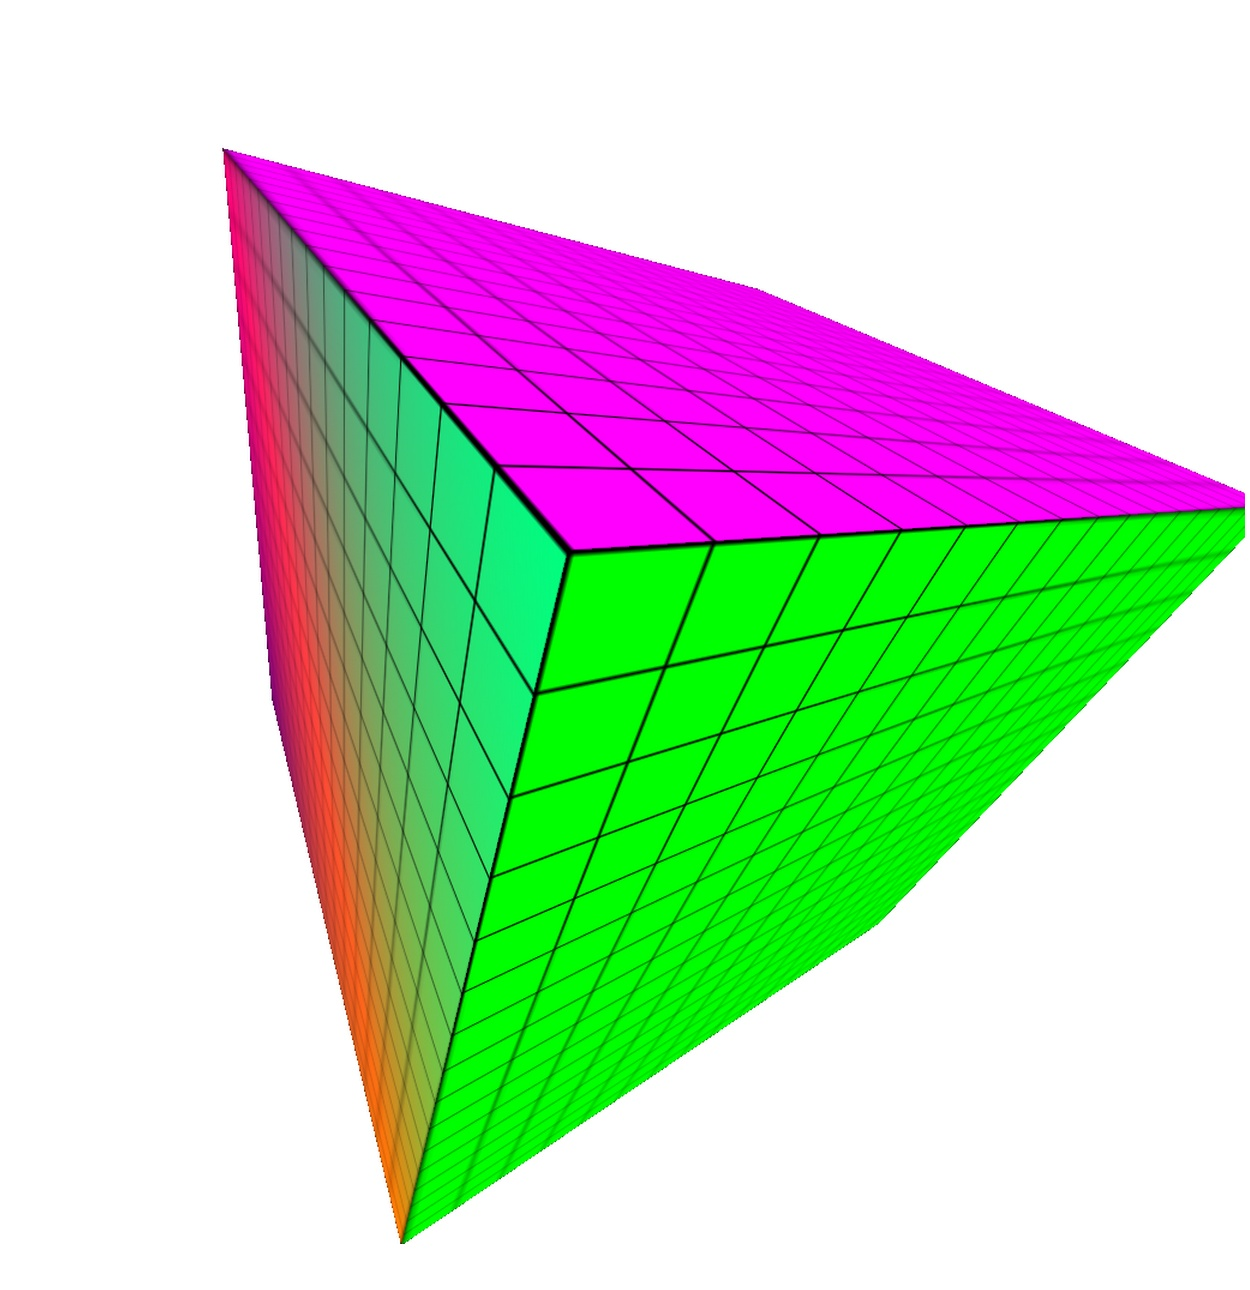
\includegraphics[width=.3\linewidth]{splat1.jpg}
  }
  \subfigure[$P_c M_c = P_s M_s$]{
    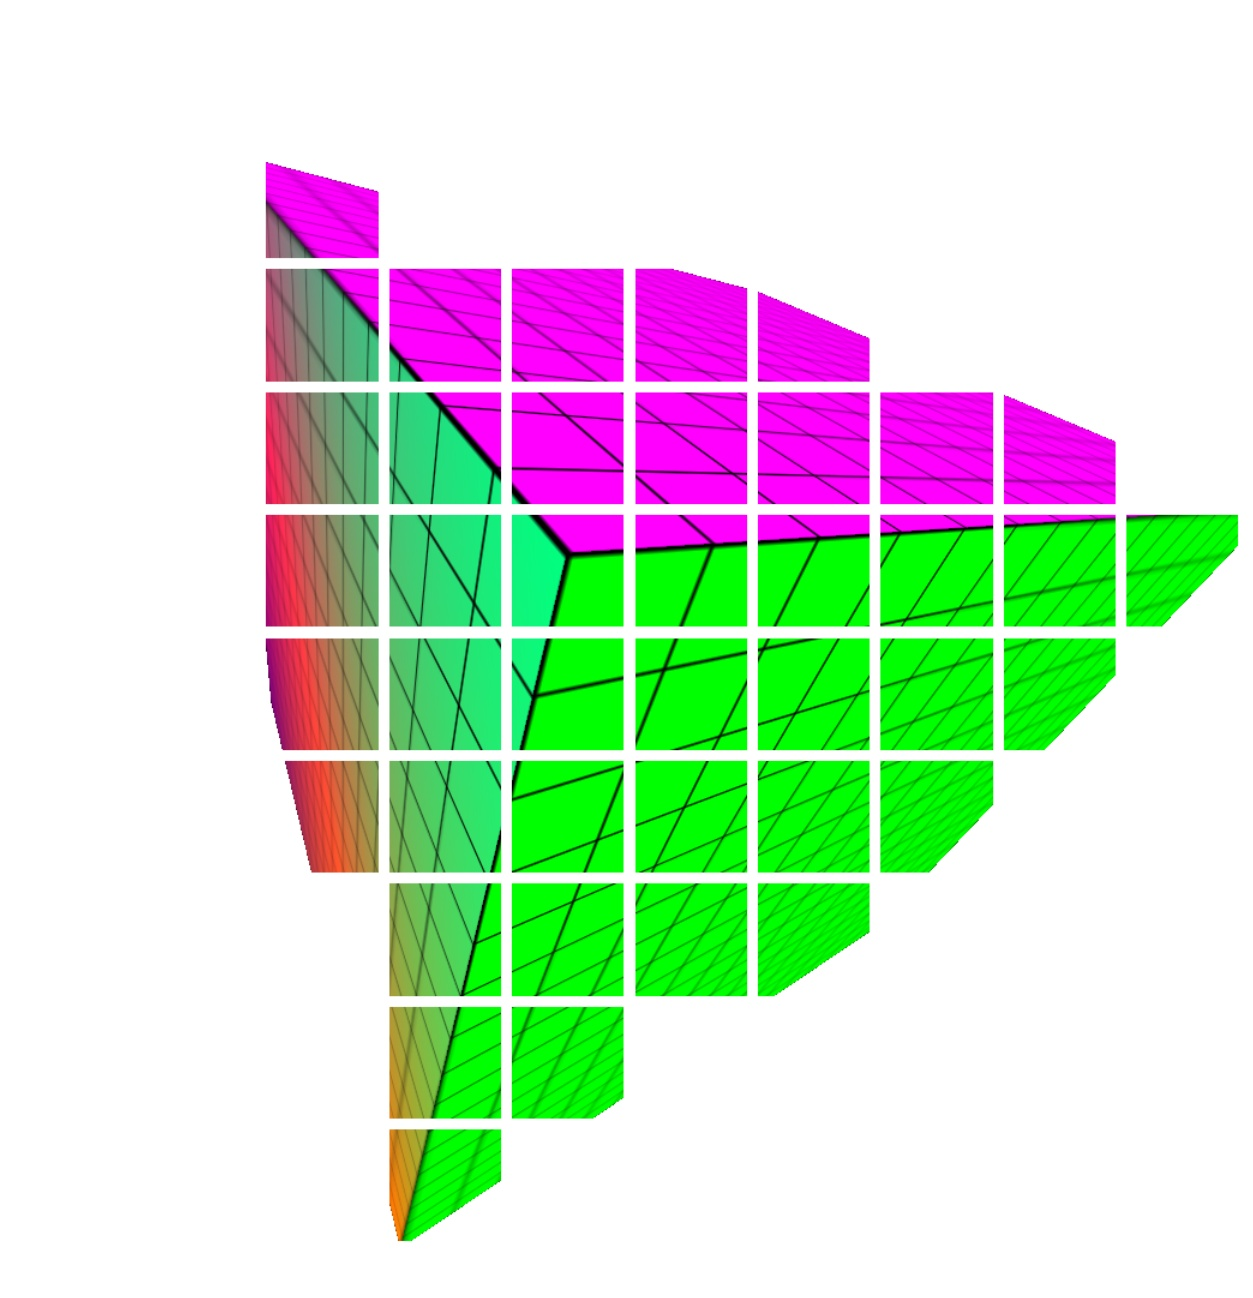
\includegraphics[width=.3\linewidth]{splat2.jpg}
  }
  \subfigure[$P_c M_c \neq P_s M_s$]{
    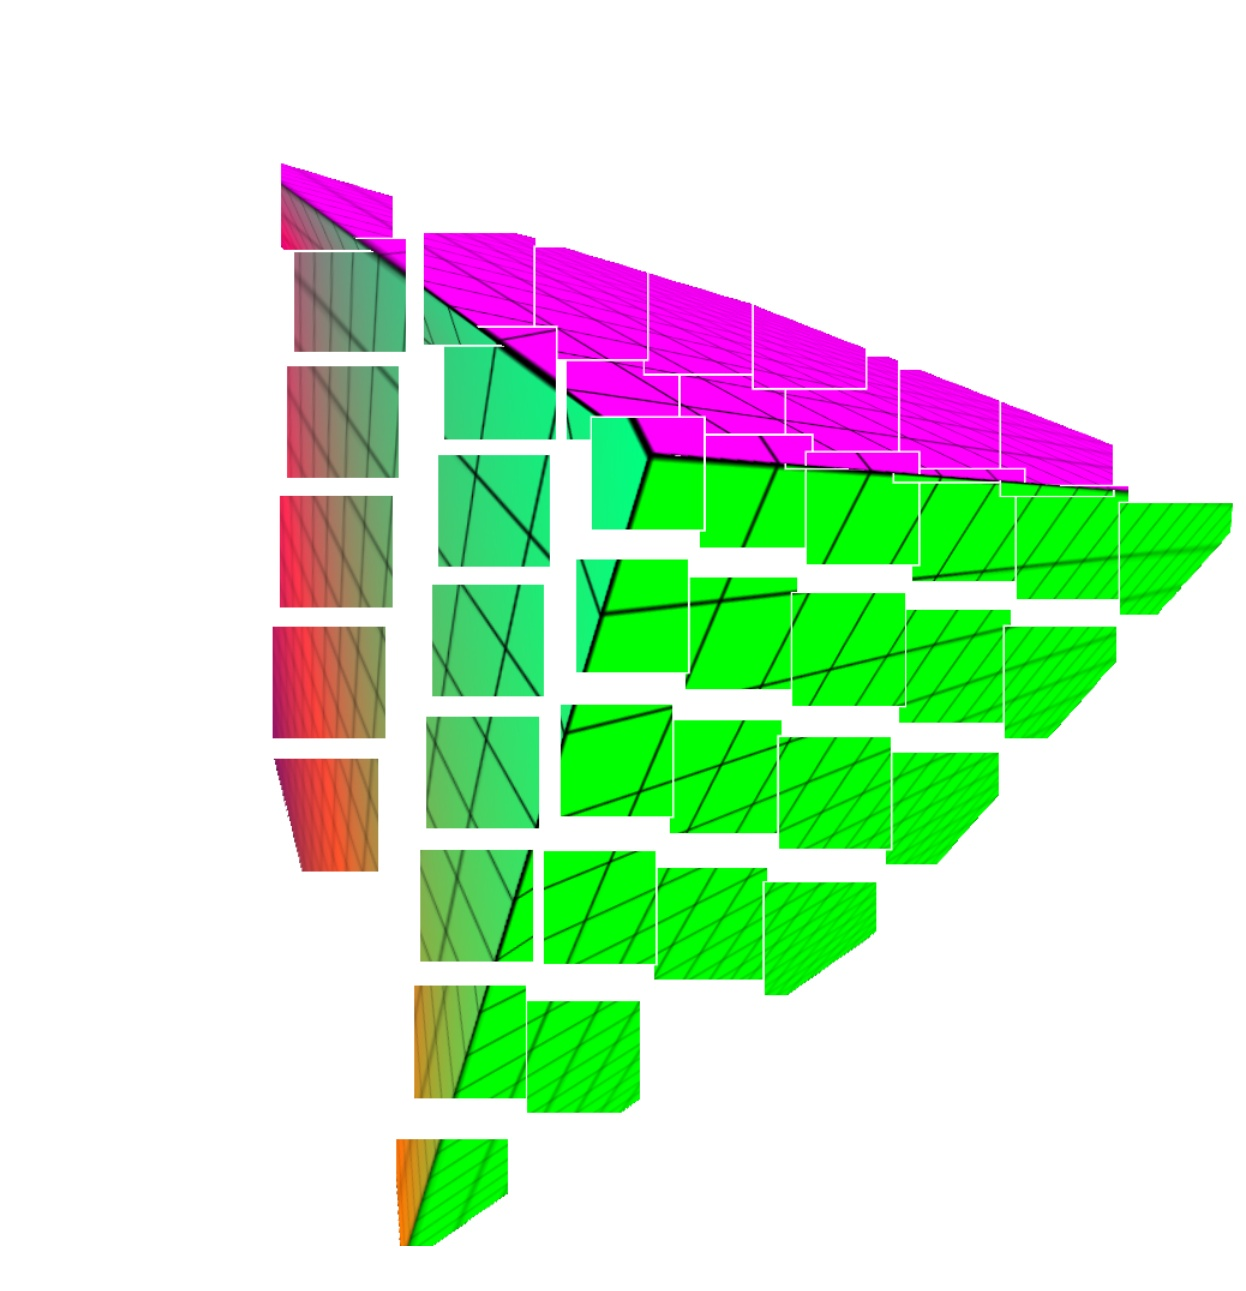
\includegraphics[width=.3\linewidth]{splat3.jpg}
  }
  \caption{\label{fig:LargeSplatsOnCorners}
           Splats for which depths are sampled on a planar region look nice on
  this region, but possibly contorted elsewhere. Notice the corner and edges
  here, where we have chosen parameters to display this effect.}
\end{figure}

When the geometry is not planar, $T$ produces the wrong result for parts of a
splat.  Two ways to remedy this could be to choose either more and smaller
splats, or introduce more complex texture transformations. Note that using a
more sophisticated texture coordinate transform may amount to performing the
same work as for more and simpler transforms. The latter may be regarded as
exactly a better ``global'' texture transform implementation.


%-------------------------------------------------------------------------
\subsubsection{Other splat considerations}
\label{sec:proxyModelReplacement}

\textbf{Splat sizing} 
Each splat should be rendered into a number of client pixels according to the
new splats' 3D position. To achieve this, we use the vectors $\sv_{\Delta x}$
and $\sv_{\Delta y}$ from the previous section, and in addition, we scale the
splats up a bit so that they overlap. Hence, we can render rectangular
window-aligned splats with less risk of getting uncovered areas when
interactively rotating and scaling the model on the client. In most cases this
removes the problem visualized in Figure~\ref{fig:LargeSplatsOnCorners}.

\textbf{Splat depth fragments}
For larger splats it makes sense to also compute and use depth fragments on the
client. The ``intra-splat'' depth values can easily be fetched from the depth
image, just as the texture is looked up for color. Not all clients support this
WebGL extension.

\textbf{Splat set replacement algorithms}
We mainly concern ourselves with proxy models defined as sets of splats, and it
makes sense to keep a set of such models on the client, then we may combine them
to cover larger ranges of client-side transformations. One can imagine a plethora of
{\em splat set replacement algorithms}, we have tested three approaches that all
retain a constant number of proxy models. The first is to replace the
one with a viewing direction differing the most from the newly received
model. The second simply replaces the oldest one in store. The third replaces a
proxy model $k$ if the replacement results in the following objective function
being reduced,
\begin{equation}
  \text{coverage} =
  \sum_{i=1}^n
    \sum_{j\neq i}^n 
      ( \angle(\textbf{camdir}_i, \textbf{camdir}_j )^2,
  \label{eq:coverage}
\end{equation}
where $n$ is the number of proxy models available, $\textbf{camdir}$ is the
direction in which the camera was looking when a particular model was generated,
and the model to be replaced is the one that minimizes~(\ref{eq:coverage}) after
replacement.


%-------------------------------------------------------------------------
\subsection{Auto-tuning}
\label{sec:autoTuning}

It is important that the process of generating and sending proxy model data from
the server itself does not slow down transmission.  There are mainly three
sources of delay for server-rendered images to the client; high latency, low
bandwidth, and slow server-rendering.  In the first case, it seems prudent to
have a good proxy model on the client, which can be used for longer time and for
a wider range of client-side transformations.  In the two other cases, it is
important for the proxy model generation/transmission to be cheap/fast, both in order
to get the proxy model to the client and keep from delaying the server-image
more than necessary. These demands are not always compatible.

We have adopted an adaptive specification of proxy model data from the server
involving a more light-weight image (lossy JPG-compression with adaptive quality
control) while interaction is ongoing.  Also, reduced resolution of the depth
buffer sent from the server is used. Another possibility is to let the client
dynamically set the number of splats, number of proxy models, etc.


%-------------------------------------------------------------------------
\section{Results and discussion}

We have tested the algorithms proposed algorithms through the Tinia 
framework~\cite{tinia}, which is a programming framework for
setting up and managing client/server based interactive visualization
applications. As client we use Google Chrome, code is written
in standard Javascript/WebGL.  The auto-proxy implementation in is invisible to the
application, so all existing Tinia-applications will have the feature
available. The algorithm is minimally intrusive in that only the depth buffer
will have to be added to the rendering output of the application. We have tested
several smaller test cases, but also on a larger oil reservoir viewer.

The reservoir viewer utilizes several GLSL shaders to render reservoir cells, boundaries,
tubular wells etc., and visualizes a 3D model that is not trivial to reduce in
complexity. It is typically also very large, so rendering it on a thin client is
prohibitive. With the automatic proxy model, we obtain interactive frame rates
with limited connection from a lightweight client. For a comparison of a
server-rendered image and a client-rendered proxy model that is slightly rotated
on the client, see again Figure~\ref{fig:FRView}. In
Figure~\ref{fig:FRView}~(a), the full server-rendered image is shown, and in~(b)
and~(c), a slightly (about 10 degrees) rotated proxy model is rendered on the
client. In~(b), parameters are chosen for best possible results, while in~(c),
we want to highlight effects, so it uses a small number of non-overlapping large
splats. One can easily spot areas not well covered, and areas where the texture
coordinate transform $T$ does not produce optimal results.



%-------------------------------------------------------------------------
\section{Conclusion and future work}

The most attractive feature of the method described is the automated generation
of the proxy model. Problems with compression and simplification of existing
geometries is bypassed altogether. The automatic proxy model implementation is
invisible to the application. There are several directions in which we would
like to follow up and improve this concept, a couple of these are,
\begin{itemize}

\item \textbf{Proxy model replacement algorithms} Obtaining good results with a minimal set of
proxy models.

\item \textbf{Depth compression} We would like to ivestigate other approaches
than just truncation, see \eg,~\cite{DBLP:journals/tvcg/Lindstrom14}.

\item \textbf{Deferred shading} With a normal map more advanced
shading could be done on the client. Such a map could also be constructed from
the depth map.

\end{itemize}


%-------------------------------------------------------------------------

\bibliographystyle{IEEEtran}




% Sample references
%\bibliography{bibtemplate_samples}

% Our references
\bibliography{egbibsample}

%-------------------------------------------------------------------------





% that's all folks
\end{document}


